
% this file is called up by thesis.tex
% content in this file will be fed into the main document

%: ----------------------- introduction file header -----------------------
%\begin{savequote}[50mm]
%Personally, I think it does help, that it makes a beneficial difference, but the scientific literature on the subject is very messy.
%\qauthor{Jeanne Petrek}
%“And upon the top of the pillars was lily work: so was the work of the pillars finished.”
%
% Bible quotes
%\end{savequote}


\chapter{Estado del Arte}
\label{cha:State of the Art}

% the code below specifies where the figures are stored
\ifpdf
    \graphicspath{{2_state_of_the_art/figures/PNG/}{2_state_of_the_art/figures/PDF/}{2_state_of_the_art/figures/}}
\else
    \graphicspath{{2_state_of_the_art/figures/EPS/}{2_state_of_the_art/figures/}}
\fi


%------------------------------------------------------------------------- 

Las competencias genéricas son las habilidades que los profesionales deben ser capaces de desempeñar independientemente de su especialización. Habilidades como el trabajo en equipo, la comunicación interpersonal, la capacidad para resolver problemas, la creatividad o el liderazgo, entre otras, son competencias que las empresas demandan hoy en día en los nuevos titulados como complemento de las competencias específicas que se les supone por la titulación que hayan estudiado. Desde un punto de vista formativo, los docentes deben integrar estas competencias en los procesos educativos, tanto en las clases tradicionales como en los entornos virtuales de aprendizaje. Y por supuesto, deben fijar mecanismos no sólo para el desarrollo de estas competencias, sino también para la evaluación de las mismas.

Un LMS es un tipo de entorno virtual de aprendizaje que almacena información de estudiantes, docentes, cursos, tareas, trabajos, etc. Estos elementos se relacionan y configuran para ofrecer al usuario una experiencia de curso virtual. Estos cursos virtuales están muy extendidos hoy en día, siendo el soporte virtual de las clases presenciales o incluso siendo el único medio donde unas clases o un curso se imparten. Las clases virtuales presentan numerosas ventajas con respecto a las clases tradicionales. Por un lado se elimina la limitación geográfica que tienen las clases tradicionales, y por otro lado la oferta y variedad de cursos ofrecidos suele ser más amplia. Además, para los estudiantes presentan otras ventajas fundamentales: en primer lugar la flexibilidad de horario, permitiéndoles compatibilizar los estudios con una vida laboral sin renunciar a crecer profesionalmente; y en segundo lugar, les permite estar en contacto permanente con otros estudiantes y docentes mediante diferentes herramientas (foros, chats, etc.)~\cite{alAjlan:2008}.

% VENTAJAS: http://oedb.org/ilibrarian/10-advantages-to-taking-online-classes/
Pero además de todo lo anterior, un entorno virtual de aprendizaje almacena una gran cantidad de información que adecuadamente presentada puede ser de gran utilidad para los docentes para analizar el trabajo de sus estudiantes~\cite{podgorelec:2011}. Cada archivo, cada acceso o cada tarea realizada por los estudiantes queda registrada en el sistema. Por desgracia, esta información no está siempre a disposición del docente, y si lo está, requiere un filtrado para poder ser utilizada~\cite{Chebil:2012}. Según el informe \emph{Making Data Work For Teachers and Students}, de la \emph{Fundación Bill \& Melinda Gates}~\cite{gates2015making}, el 67\percentage{ }de los docentes no están del todo satisfechos con el aprovechamiento que sacan de los datos y las herramientas que utilizan regularmente. Además, en este mismo informe se extrae que el 78\percentage{ }de los docentes cree que los datos les ayudarían a validar lo que sus estudiantes son y lo que pueden conseguir.   

La información almacenada en el registro de un entorno virtual de aprendizaje podría darnos indicadores sobre cómo actuarían los estudiantes en situaciones laborales reales y podría utilizarse para medir cómo de eficaz es un estudiante trabajando en equipo, cómo se planifica un estudiante a la hora de realizar sus tareas o si lidera eficazmente un grupo. ¿Podríamos entonces afirmar que los registros de actividad de un entorno virtual de aprendizaje pueden utilizarse para evaluar competencias genéricas? Para responder a esta cuestión y establecer la base teórica sobre la que se sustenta esta tesis doctoral se presenta un \emph{estudio de mapeo sistemático} (SMS, del inglés \emph{Systematic Mapping Study}). Un SMS es una amplia revisión de los estudios primarios en un área específica cuyo objetivo es identificar alguna evidencia sobre el tema y cuyo punto de partida inicial serán las preguntas de investigación que se definirán en el siguiente apartado.
\nomenclature{SMS}{Estudio de mapeo sistemático (Systematic Mapping Study)}

\section{Preguntas de investigación del SMS}

El objetivo principal de esta tesis doctoral (presentado en la sección~\ref{sec:objetivos}) es:

\begin{quote}
\emph{Proponer un método para evaluar a los estudiantes en el desempeño de sus competencias genéricas mediante indicadores procedentes de los registros de actividades de aprendizaje.}
\end{quote}

Para abordar este objetivo ha de conocerse primero el estado del arte, dando respuesta para ello a diferentes preguntas de investigación tales como cuáles son las competencias genéricas que se han evaluado haciendo uso de métodos y técnicas informáticas, cuáles son esos métodos y si se están usando para este fin los registros de actividad de los entornos virtuales de aprendizaje.

\bigskip
Por tanto, partiendo del objetivo principal, se definen las siguientes preguntas de investigación para el SMS:
\begin{itemize}
\item SMS1. ¿Qué competencias se han evaluado de forma automática o asistida por ordenador a partir de la actividad de los estudiantes en los entornos virtuales de aprendizaje?
\item SMS2. ¿Qué métodos se utilizan para evaluar competencias genéricas en entornos virtuales de aprendizaje?
\item SMS3. ¿Qué técnicas se utilizan para evaluar competencias genéricas a partir de los registros de actividad de un entorno virtual de aprendizaje?
\end{itemize}

\section{Metodología}

 Un SMS es una amplia revisión de los estudios primarios en un área específica cuyo objetivo es identificar alguna evidencia sobre el tema. Este estudio se basa en las directrices de la metodología propuesta por Kitchenham~\cite{keele2007guidelines} sobre cómo se deben planificar, ejecutar y presentar los resultados de una revisión de la literatura en ingeniería del software. Y en particular, para este trabajo se ha utilizado la propuesta de Petersen~\cite{Petersen:2008}, que describe una serie de etapas con las que llevar a cabo una revisión de la literatura a partir de un mapeo sistemático. Se comenzará describiendo un protocolo de revisión, los motores de búsqueda y los términos de búsqueda a emplear.

\paragraph*{Protocolo de revisión}
La definición del protocolo de revisión requiere la especificación de una serie de pasos para obtener la bibliografía de nuestro estudio. Los pasos a seguir son los siguientes:
\begin{enumerate}
\item Selección de motores de búsqueda (sección \ref{sec:MotoresBusqueda}).
\item Definición de los términos de búsqueda (sección \ref{sec:TerminosBusqueda}).
\item Determinación de los criterios de selección (sección \ref{sec:CriteriosBusqueda}).
\item Clasificación para la extracción de datos (sección \ref{sec:EsquemaBusqueda}).
\end{enumerate}

%Comenzaremos indicando los motores de búsqueda que vamos a utilizar, qué términos de búsqueda utilizaremos en dichos motores y las herramientas de soporte a la revisión. Además se mostrarán qué criterios de inclusión de la bibliografía se siguen y el procedimiento de selección.

\paragraph*{Motores de búsqueda}
\label{sec:MotoresBusqueda}
Para encontrar la bibliografía, se realizarán consultas en las siguientes bibliotecas digitales: 
\begin{itemize}
\item Web of Science
\item Wiley Online Library
\item Science Direct
\item IEEE Digital Library (Xplore)
\end{itemize}

\paragraph*{Términos de búsqueda}
\label{sec:TerminosBusqueda}
Existen diversos términos que pueden utilizarse para referirse a la evaluación de competencias genéricas de manera automatizada o asistida. Por la naturaleza de nuestro trabajo, debemos contemplar siempre en las palabras de búsqueda los términos \emph{assessment} y \emph{generic skills} o \emph{generic competences}. Realizar la búsqueda por el término \emph{Assessment of generic skills} o \emph{assessing generic skills} devolvía muy pocos resultados. Por ejemplo, en la \emph{Wiley Online Library} la búsqueda del término exacto \emph{generic skills assessment} devolvió un único resultado. Sin embargo, debilitar la búsqueda con términos como \emph{generic competences} o \emph{generic skills} junto con la palabra \emph{assessment} daba un número de resultados muy elevado. En la misma biblioteca, buscar por los términos \emph{``generic skills`` and student and assessment} nos devolvía 609 resultados. En primera instancia se probó añadiendo términos como  \emph{E-Learning}, \emph{computer-assisted} o \emph{mobile learning}. Sin embargo, incluir términos de este tipo reducía también drásticamente el número de resultados obtenidos en la búsqueda, no llegando a obtenerse bibliografía más significativa que si no se incluían. Por tanto, a tenor de las pruebas se decide eliminar de la búsqueda ese tipo de términos. La combinación de los términos de búsqueda empleados en la investigación, así como a los motores de búsqueda que fueron aplicados en cada una pueden observarse en la tabla \ref{tab:ResumenBusqueda}. Los términos de búsqueda se han empleado en todos los campos (título, resumen, texto, etc.).

%Por otro lado, sí se incluyen acrónimos de diferentes entornos virtuales relacionados con las TEL, como son: \emph{TEL}, \emph{LMS}, \emph{ICT} (Information and Communications Technology), \emph{CBI} (Content-Based Instruction). Y tras varias pruebas, se descartan también de la búsqueda términos como `\emph{ICE} (Integrated Collaboration Environment) y \emph{CSCL} (Computer Supported Collaborative Learning), debido a que son términos que en conjunción con los términos principales de nuestra búsqueda no suelen aparecer y los resultados de estas búsquedas eran nulos. Un ejemplo de esto se refleja en una de las consultas realizadas en \emph{Scopus}, dónde los términos \emph{((``student assessment`` OR ``assessment of students``) AND (``generic skills`` OR ``generic competences``)) AND CSCL} no devolvían ningún resultado. 

\begin{table}
  \begin{center}
  \setlength\tabcolsep{2.5pt}
  \begin{tabular}{| L{2.9cm} | L{4.2cm} | L{2.8cm} | R{2.8cm} |}
    \hline
    FUENTE & TÉRMINOS DE BÚSQUEDA & PUBLICACIÓN & RESULTADOS \\
    \hline
    \hline
    Web of Science & ((``generic competences`` OR ``generic skills``) AND assessment) & Journals & 138 \\
    \hline
    Wiley Online Library & ``generic competences`` AND assessment & Journals and Conferences & 50 \\
    \hline
    Science Direct & (``generic competences``) AND assessment) & Journals & 71 \\
    \hline
    IEEE Digital Library (Xplore) & ((``generic competences``) AND assessment) & Journals and Conferences & 54 \\
    \hline
    \hline
    \multicolumn{3}{|r|}{TOTAL} & 313\\
    \hline

%    Wiley Online Library & assessment AND ``generic competences`` OR ``generic skills`` AND (TEL OR ICT OR CBI) & in All Fields\\
%    World Scientific Net & ``generic competences`` OR ``generic skills`` AND assessment & Anywhere in article\\
%    Springer & (``generic skills`` OR ``generic competences``) AND  students AND (TEL OR CBI OR ICT) & All fields (Including full text)\\
%    ACM Digital Library & (assessment and ``generic skills``) and (TEL or LMS or ICT or CBI) & Any field (title, abstract, review)\\
%    ACM Digital Library & (assessment and ``generic competences``) and (TEL or LMS or ICT or CBI) & Any field (title, abstract, review)\\
%	  IEEE Digital Library (Xplore) & (((TEL or LMS or ICT or CBI) AND (``generic skills`` OR ``generic competences``)) AND assessment) & Full text and metadata\\
%    Scopus & (((TEL or LMS or ICT or CBI) AND (``generic skills`` OR ``generic competences``)) AND assessment) & All fields (Including full text)\\
    \hline
  \end{tabular}
\end{center}
\caption{Resumen de búsqueda de bibliografía}
\label{tab:ResumenBusqueda}
\end{table} 

\subsection{Criterios de selección}
\label{sec:CriteriosBusqueda}
Para determinar si un trabajo debía formar parte de nuestra selección de estudios primarios se leyó el título, el resumen y las palabras clave. Cuando esto no era suficiente se complementaba la lectura anterior con una somera la lectura del artículo completo, y más detallada de la introducción y las conclusiones.
Nuestra búsqueda se centró en la localización de los trabajos que, habiendo sido obtenidos en el proceso de búsqueda anterior, vayan en línea con nuestro estudio y puedan ayudarnos a resolver las preguntas de investigación. Para ello, se realizó la proyección de los trabajos seleccionados utilizando los siguientes criterios de exclusión:
\begin{itemize}
\item Incluido (\emph{included}): trabajo relacionado con nuestra investigación.
\item Fuera del tema (\emph{off Topic}): trabajo no relacionado directamente con nuestra investigación. Son trabajos que satisfacen los criterios de búsqueda, pero cuya contribución no está directamente relacionada con la temática de este estudio. La mayoría de artículos descartados en este bloque consisten en experiencias que trabajan o mejoran alguna competencia genérica en los estudiantes, pero no mencionan si después el desempeño en la competencia se mide de alguna forma, y si por el contrario sí realizan una medición, lo hacen sin apoyo alguno de la tecnología.
\item Idioma no disponible (\emph{Unsupported Language}): trabajo escrito en un idioma diferente al inglés o español. La mayoría de los textos son en inglés, por lo que este criterio de descarte apenas es utilizado.
\item Duplicado (\emph{duplicated}): trabajos cuya contribución principal está recogida en otros trabajos ya incluidos. 
\item No leído (\emph{unread}): trabajo que no ha podido ser leído. Son textos que no han sido leídos al no estar disponible en las bibliotecas digitales a las que se tiene acceso desde la Universidad de Cádiz ni se ha podido encontrar por otros medios (petición por correo a los autores, búsqueda en repositorios abiertos de Internet, etc.).
\end{itemize}

\subsection{Esquema para la extracción de datos}
\label{sec:EsquemaBusqueda}

Para la extracción de la información se han dividido los trabajos de acuerdo a los siguientes tres aspectos: tipo de investigación, tipo de contribución y ámbito de aplicación de la investigación. A continuación se detalla esta clasificación.

\subsubsection*{Tipo de investigación}
Esta clasificación hace referencia al tipo de trabajo de investigación llevado a cabo por los investigadores. Existen diferentes enfoques para la clasificación de los trabajos según el tipo investigación que desarrollan. Algunos de estos sistemas de clasificación son los propuestos por Wieringa \cite{Wieringa:2005} y Hevner \cite{Hevner:2004}. Usamos el primero, ya que es el recomendado en el SMS descrito por Petersen \cite{Petersen:2008}.
\begin{itemize}
\item Solución propuesta (\emph{proposal of solution}): se propone una solución para un problema; la solución puede ser innovadora o una extensión significativa de una técnica existente. Los posibles beneficios y la aplicabilidad de la solución se demuestran por un pequeño ejemplo o una buena línea de argumentación.
\item Investigación por validación (\emph{validation research}): las técnicas investigadas son nuevas y todavía no se han aplicado en la práctica. Estas técnicas podrían ser por ejemplo los experimentos, es decir, el trabajo realizado en un laboratorio.
\item Investigación por evaluación (\emph{evaluation research}): las técnicas se aplican en la práctica y se lleva a cabo una evaluación de la técnica. Se muestra cómo se implementa la técnica en la práctica (implementación de la solución) y cuáles son las consecuencias de la aplicación en términos de ventajas y desventajas (evaluación de implementación).
\item Artículos de experiencia (\emph{experience papers}): trabajos que explican qué y cómo algo se ha llevado a cabo en la práctica. Basado en la experiencia personal de los autores.
\item Artículos de opinión (\emph{opinion papers}): estos trabajos expresan la opinión personal de alguien acerca de la bondad o viabilidad de una determinada técnica, o sobre cómo se debería implementar dicha técnica.
\item Trabajos filosóficos (\emph{philosophical papers}): estos trabajos esbozan una nueva forma de ver las teorías existentes, estructurando el campo en forma de una taxonomía o un marco conceptual.
\end{itemize}

\subsubsection*{Tipo de contribución}
En este apartado se clasifican los trabajos según el tipo de contribución que realizan estos al ámbito en el que se desarrollan. Una vez realizado el estudio sistemático de la literatura y habiendo seleccionado los artículos, se realiza una clasificación en base a su aportación.
 
Lamentablemente, el uso de algunos términos puede ser confuso, debido a las diversas interpretaciones del mismo que hacen distintos autores. Algunos de estos términos son framework, modelo, estrategia, proceso, procedimiento, método o metodología. Nuestra interpretación es la siguiente:
\begin{itemize}
\item Modelo (\emph{model}): es una representación de procesos, modelos o sistemas pertenecientes a un supra-sistema, cuyo fin es el análisis de interacción de ellos para mantener una relación flexible que les permita cumplir su función particular y cumplir la función de dicho supra-sistema.
\item Método (\emph{method}): contempla aquellos trabajos cuya contribución sea descrita por los autores como una serie de pasos.
\item Herramienta (\emph{tool}): se utiliza para los artículos que presentan un software independiente o una extensión de algún otro programa.
\item Framework (\emph{framework}): aquí se consideran aquellos trabajos que contribuyen con una combinación de los elementos anteriores (es decir, con un modelo, un proceso y una herramienta).
\item Técnica (\emph{technique}): un procedimiento utilizado para llevar a cabo una actividad o tarea específica. Podría venir acompañado de una herramienta de apoyo.
\end{itemize}

\subsubsection*{Ámbito de aplicación de la investigación}
Además de las clasificaciones anteriores, es necesario extraer más información acerca de los conceptos que representan la contribución de investigación. Para ello se recopila información sobre el ámbito y la manera en la que se realiza la evaluación de competencias en cada contribución. Una vez identificada esta información, se agrupan según sus similitudes, quedando finalmente la siguiente clasificación:
\begin{itemize}
\item Evaluación del docente (\emph{teacher assessment}): el docente evalúa el desempeño de los estudiantes en una o varias competencias genéricas de manera asistida o semi-asistida por un sistema informático.
\item Evaluación entre iguales y autoevaluación (\emph{peer and self-assessment}): en estos trabajos los estudiantes se encargan de todo o de parte del proceso de evaluación, ya sea evaluando su propio trabajo (autoevaluación) o el de sus compañeros (evaluación entre iguales), y utilizando para ello algún tipo de sistema informático. Los investigadores animan a los docentes a utilizar este tipo de evaluación ya que ayuda a los estudiantes a reflexionar sobre su propio aprendizaje y favorecer el aprendizaje colaborativo en el aula~\cite{chen2010implementation}.
\item Herramientas de evaluación semiautomática (\emph{semiautomatic assessment tools}): en esta categoría se recogen trabajos que automatizan en parte el proceso de evaluación de competencias.
\end{itemize}

\subsection{Visualización y análisis de los datos}
Tras obtener los estudios primarios, hay una etapa de análisis, donde se resumen los datos extraídos para responder a las preguntas de investigación planteadas. El análisis de los resultados se centra en el estudio de las publicaciones para cada categoría y por lo tanto, en la determinación del grado de cobertura de cada categoría. Esta información generalmente se resume en tablas y gráficos. Otro método utilizado en nuestro estudio es la combinación de diferentes categorías (por ejemplo, el ámbito de investigación contra el tipo contribución) y su representación se muestra en un mapa sistemático en forma de gráfico de burbujas.

En el siguiente capítulo se presentan los resultados obtenidos.

\section{Resultados}

A continuación se muestran los resultados del estudio. Comienza el capítulo con la localización de los estudios primarios, para continuar con la extracción de los datos de estudio, mostrándose varios gráficos y tablas que justifican la información mostrada. Finalmente se categorizan los estudios y se muestra el esquema de clasificación resultante.

\subsection{Localización de la literatura}

En la tabla \ref{tab:ResumenBusqueda} se muestran las búsquedas realizadas en las bibliotecas digitales más importantes en ingeniería informática, los términos de búsqueda utilizados y el número de documentos obtenidos. En cada biblioteca, se utilizaron los formularios de búsqueda avanzada y los resultados fueron obtenidos a fecha 21 de agosto de 2015. Toda la información resultante de las búsquedas de este SMS está disponible para su consulta \footnote{\url{https://goo.gl/rzTCHN}}.

%\footnote{http://sms.antoniobalderas.es}.

En total se recopilaron 313 trabajos. El número de estudios primarios resultante (después de aplicar criterios de selección y exclusión) fue de 30 trabajos (menos de un 10\percentage{ }del total de trabajos recopilados). Además, 268 trabajos se catalogaron como ``fuera del tema''. Los resultados de esta clasificación pueden verse en la tabla \ref{tab:ResumenSelecccionResultados}. A tenor de los resultados ofrecidos, y sobre todo del número de trabajos descartados, el lector puede pensar que se debieron añadir términos informáticos entre los criterios de búsqueda. Sin embargo, el número de términos informáticos que se podrían añadir a las búsquedas era muy amplio y determinados trabajos que han sido recopilados en este trabajo hubieran quedado fuera en ese caso porque hubiera sido imposible tener todos los términos en cuenta. Además, el hecho de que las bases de datos utilizadas sean específicas de informática y computación es garantía suficiente de que sus aportaciones deben ser en su mayoría basadas en tecnología.

\begin{table}
  \begin{center}
  \begin{tabular}{| m{4cm} | r | r |}
    \hline
    CRITERIO & TRABAJOS & PORCENTAJE\\
    \hline
    \hline 
    Incluido & 30 & 9,58\percentage \\
    \hline
    Fuera del tema & 268 & 85,62\percentage \\
    \hline
    Idioma no disponible & 0 & 0,00\percentage \\
    \hline
    Duplicado & 10 & 3,20\percentage \\
    \hline
    No leído & 5 & 1,60\percentage \\
    \hline
    \hline
    TOTAL & 313 & 100,00\percentage \\
    \hline
  \end{tabular}
\end{center}
\caption{Clasificación de trabajos tras aplicar los criterios de selección y exclusión}
\label{tab:ResumenSelecccionResultados}
\end{table} 

\subsection{Extracción de datos}

Aunque las tecnologías entraron a formar parte de la vida académica hace ya varios años, no es hasta 2013, con la tercera generación de herramientas de medición educativa según el marco de la Comisión Europea (\emph{Generation 3: continuous integrated assessment}) \cite{Redecker:2013}, cuando se comienzan a integrar la evaluación en las herramientas de aprendizaje. Es a partir de entonces cuando conceptos como \emph{Data Mining and analysis}, \emph{Behavioural tracking} and \emph{Learning analytics} comienzan a usarse. Tanto en la tabla \ref{tab:ResumenAniosResultados} como en la figura \ref{fig:PublicacionesAnuales} puede verse la distribución de la producción de la selección primaria a lo largo de los años. La mayoría de los seleccionados se pueden localizar en los últimos años. Véase como 16 de estos trabajos (53,33\percentage) fueron publicados entre 2013 y 2015.

% Quitada coma tras véase (, véase) por mal uso. Estará mejor un punto y seguido?

\begin{table}
  \begin{center}
  \begin{tabular}{| c | c | r |}
    \hline
    AÑOS & RESULTADOS & PORCENTAJE\\
    \hline    
    \hline
    2007 & 2 & 7\percentage\\
    \hline
    2008 & 2 & 7\percentage\\
    \hline
    2009 & 2 & 7\percentage\\
    \hline
    2010 & 3 & 10\percentage\\
    \hline
    2011 & 4 & 13\percentage\\
    \hline
    2012 & 1 & 3\percentage\\
    \hline
    2013 & 9 & 30\percentage \\
    \hline
    2014 & 4 & 13\percentage\\
    \hline
    2015 & 3 & 10\percentage \\
    \hline
  \end{tabular}
\end{center}
\caption{Cantidad de trabajos publicados cada año}
\label{tab:ResumenAniosResultados}
\end{table}

\begin{figure}
  \begin{center}
    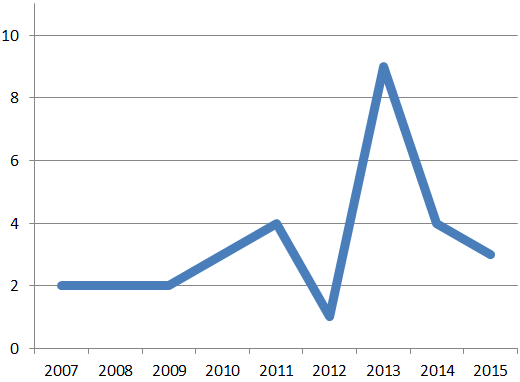
\includegraphics[scale=0.4]{PublicacionesAnualesSinLeyenda.png}
  \end{center}
  \caption{Distribución de las publicaciones por años}
  \label{fig:PublicacionesAnuales}
\end{figure}


%\subsection{Características de los trabajos seleccionados}

Todos los trabajos seleccionados evalúan una o varias competencias genéricas utilizando algún método, técnica e instrumento de evaluación. Para el esquema de clasificación se concreta para cada trabajo las competencias que evalúa y con qué método, técnica y herramienta lo hace. A continuación se describen para cada una de estas características los valores que aparecerán en la revisión para que queden definidos todos los términos que aparecen en el capítulo del esquema de clasificación.

\subsubsection*{Competencias genéricas}

En la tabla~\ref{tab:CompetenciasGenericas} se muestran las competencias genéricas que se evalúan en los trabajos seleccionados. De esta manera, se unifica la denominación de las competencias, ya que en ocasiones los autores se refieren a las mismas competencias de diferentes denominaciones. En la primera columna se muestra la denominación corta que se utilizará para referirnos a cada competencia. Al clasificar los artículos se han utilizado las competencias genéricas definidas en el \emph{Tuning Educational Structures in Europe}~\cite{gonzalez2005tuning}. 


\begin{landscape}
\pagestyle{empty}
  \begin{center}
\begin{longtable}{| L{6cm} | L{16cm} |}
    \hline
    COMPETENCIA & DESCRIPCIÓN \\
    \hline
    \hline
    Análisis & Capacidad de abstracción, análisis y síntesis~\cite{gonzalez2005tuning}.\\
    \hline
    Aprendizaje permanente & Marco constituido por el aprendizaje formal, no formal e informal, que aspira a la adquisición de conocimiento para alcanzar el máximo desarrollo de la personalidad y de las destrezas profesionales en las diferentes etapas de la vida~\cite{bernheim2010educacion}. \\
    \hline
    Comunicación & Habilidad para comunicarse de manera tanto oral como escrita en la lengua materna~\cite{gonzalez2005tuning}. \\
    \hline
    Creatividad & Capacidad para crear nuevas ideas~\cite{gonzalez2005tuning}. \\
    \hline
    Cultural & Aprecio y respeto por la diversidad y la multiculturalidad~\cite{gonzalez2005tuning}. \\
    \hline
    Emprendimiento & Capacidad para tomar la iniciativa y espíritu de empresa~\cite{gonzalez2005tuning}. \\
    \hline
    Gestión de proyectos & Habilidades para diseñar y gestionar proyectos~\cite{gonzalez2005tuning}. \\
    \hline
    Habilidades interpersonales & Capacidad de la persona para comunicarse e interactuar con otras personas~\cite{gonzalez2005tuning}. \\ % De aquí: http://www.skillsyouneed.com/interpersonal-skills.html
    \hline    
    Investigación & Capacidad para llevar a cabo la investigación en un nivel apropiado~\cite{gonzalez2005tuning}.  \\
    \hline 
    Lengua extranjera & Capacidad de los estudiantes para comunicar sus ideas en un segundo idioma~\cite{gass2013second}. \\
    \hline
    Liderazgo & Habilidad para motivar a la gente y conducirlos hacia un objetivo común~\cite{gonzalez2005tuning}. \\
    \hline
    Pensamiento crítico & Habilidad para interpretar, analizar y evaluar ideas y argumentos~\cite{fisher2011critical}. \\
    \hline
    Planificación y gestión del tiempo & Capacidad de planificar y gestionar el tiempo de manera efectiva~\cite{gonzalez2005tuning}. \\
    \hline
    Resolución de problemas & Habilidad para identificar, plantear y resolver problemas~\cite{gonzalez2005tuning}. \\
    \hline
    Responsabilidad & Capacidad para actuar con responsabilidad social y conciencia cívica~\cite{gonzalez2005tuning}. \\
    \hline
    TIC & Habilidades en el uso de las tecnologías de la información y de la comunicación~\cite{gonzalez2005tuning}. \\
    \hline
    Toma de decisiones & Capacidad para tomar decisiones razonadas~\cite{gonzalez2005tuning}. \\
    \hline
    Trabajo autónomo & Capacidad para trabajar de forma autónoma~\cite{gonzalez2005tuning}. \\
    \hline
    Trabajo en equipo & Trabajo realizado por un conjunto de personas en aras de un objetivo común~\cite{dixon1992teamwork}. \\
    \hline
\caption{Competencias genéricas}
\label{tab:CompetenciasGenericas}
\end{longtable} 
\end{center}
\end{landscape}
\pagestyle{fancy}

\subsubsection*{Métodos}
\label{sec:methods}
En cada uno de los trabajos seleccionados se llevaba a cabo un método de evaluación. A partir de la descripción que realizaban los autores sobre el proceso de evaluación realizado, cada trabajo ha sido clasificado dentro de alguno de los métodos que a continuación se detallan:

\begin{itemize}
\item Evaluación formativa (\emph{formative assessment}): proceso utilizado por docentes y estudiantes para identificar y reaccionar al aprendizaje de los estudiantes con el fin de mejorar dicho aprendizaje mientras éste tiene lugar~\cite{bell2001characteristics}. Es una parte integral del proceso educativo cuyo objetivo es proporcionar información de manera sistemática y continua sobre el propio proceso.
\item Evaluación sumativa (\emph{summative assessment}): método que mide el grado de éxito de los estudiantes a la hora de alcanzar los criterios utilizados para medir los objetivos de aprendizaje fijados para el curso o módulo. Se utiliza para cuantificar los logros y proporcionar información para la aptitud o no del evaluado de pasar al siguiente nivel o módulo~\cite{tyler1967perspectives}.
\item Evaluación auténtica (\emph{authentic assessment}): evaluación en la que las tareas están estrechamente alineadas con lo que el estudiante experimentará en el mundo laboral. Este tipo de evaluación está diseñado para desarrollar en los estudiantes habilidades y competencias en paralelo al desarrollo académico~\cite{gulikers2004five}.
\item Evaluación diagnóstica (\emph{diagnostic assessment}): al igual que la evaluación formativa, es una evaluación que pretende mejorar la experiencia del estudiante y su nivel de éxito. La diferencia con respecto a la evaluación formativa radica en que mientras que la evaluación diagnóstica se realiza antes de que comience el proceso educativo con la intención de conocer lo que el estudiante ya sabe y las dificultades que se encontrará, la formativa se realiza durante el proceso~\cite{huhta2008diagnostic}.
\item Evaluación dinámica (\emph{dynamic assessment}): mide lo que el estudiante logra cuando se le imparten algunas nociones sobre un tema o campo desconocido. Puede ser útil para evaluar el potencial en un tema concreto en ausencia de un logro anterior relevante, o para evaluar el potencial de aprendizaje general para los estudiantes que tienen un contexto desfavorecido. A menudo se utiliza antes de que el cuerpo principal de la enseñanza~\cite{lidz1987dynamic}.
\item Evaluación sinóptica (\emph{synoptic assessment}): estimula a los estudiantes a combinar elementos de su aprendizaje desde diferentes partes de un programa para mostrar el conocimiento acumulado y la comprensión de un tema o materia especifica. Una evaluación sinóptica normalmente permite a los estudiantes mostrar su capacidad de integrar y aplicar sus habilidades, conocimientos y entendimiento con amplitud y profundidad en el tema. Puede ayudar a evaluar la capacidad de los estudiantes de aplicar el conocimiento y la comprensión obtenida en una parte del programa para mejorar sus comprensión en otras partes del programa o a lo largo del mismo. La evaluación sinóptica puede formar parte de otras formas de evaluación~\cite{qaa2006quality}.
\item Evaluación con referencia al criterio (\emph{criterion referenced assessment}): los logros de cada estudiante se juzgan con respecto a criterios específicos, sin tener en cuenta lo logrado por otros estudiantes. En la práctica, la comparación con otros sujetos puede afectar al enjuiciar si un criterio específico se ha cumplido o no~\cite{dunn2002seeking}.
\item Evaluación ipsativa (\emph{ipsative assessment}): esta evaluación se realiza con respecto al nivel previo del estudiante. Puede medir el nivel con el que un estudiante ha desempeñado una tarea particular con respecto a su propio nivel medio de desempeño, con respecto a su mejor trabajo o con respecto a su trabajo más reciente. La evaluación ipsativas se suele correlacionar con el esfuerzo, para promover la recompensa al trabajo y mejorar la motivación para aprender~\cite{hughes2011towards}.
\end{itemize}

\subsubsection*{Técnicas}
\label{sec:techniques}

En cada uno de los trabajos seleccionados se utilizó alguna técnica para llevar a cabo alguno de los métodos de evaluación anteriormente descritos. A continuación se describen el conjunto de técnicas que aparecen en estos trabajos:

\begin{itemize}
\item \emph{Observación sistemática}: técnica para la recolección de datos sobre el aprendizaje basada en inspección y estudio esencialmente descriptivo de la actividad, evento o hecho realizado por el estudiante a evaluar.  Algunos instrumentos típicos son rúbricas, guías de observación y listas de comprobación.
\item \emph{Pruebas escritas}: instrumento de medición cuyo propósito es que el estudiante demuestre la adquisición de un aprendizaje cognitivo, o el desarrollo progresivo de una destreza o habilidad. Por sus características, requiere contestación escrita por parte del estudiante~\cite{rojas2008prueba}. Algunos instrumentos que se utilizan en esta técnica son los exámenes escritos y los cuestionarios.
\item \emph{Pruebas orales}: interacción oral evaluador-evaluado mediante la que el evaluado busca acreditar conocimiento sobre un tema determinado ante uno o varios evaluadores que a vez utilizarán esta exposición para calificar al evaluado en el desempeño de alguna competencia. 
\item \emph{Indicadores basados en logros}: indicadores que marcan si un resultado final o logro se ha alcanzado y para determinar así el grado en que cada competencias ha sido desarrollada. El propósito es conseguir que los estudiantes desarrollen competencias, y los indicadores son el recurso para evaluar dicho desarrollo. Esta técnica es típica en los juegos serios, en donde las distintas fases o etapas del juego con sus correspondientes logros se mapean a indicadores del nivel de desempeño de competencias~\cite{balta2016coddii}.
\item \emph{Indicadores de trabajo en entornos virtuales de aprendizaje}: indicadores del proceso de desarrollo del trabajo realizado por los estudiantes (no del trabajo final en sí). Encontramos estas técnicas en experimentos en los que tras haber trabajado los estudiantes en diferentes actividades del entorno virtual de aprendizaje son evaluados del desempeño en diferentes competencias a partir de los registros de interacción de estos estudiantes con el propio entorno. 
\item \emph{Actividades sin determinar}: se utiliza este término para referirnos a las técnicas que se han utilizado en trabajos en los que se indica que se han evaluado actividades pero no se menciona explícitamente el cómo. Por contexto pueden ser tanto actividades del entorno virtual de aprendizaje como actividades presenciales. No se presta atención a cómo son y cómo se evalúan esas actividades en particular, sino a que después se toma la calificación de cada actividad y de una u otra forma se mapea a la evaluación de alguna competencia. Quizás se usen rúbricas, cuestionarios o entrevistas, pero o no se mencionan o si lo hacen no está directamente relacionado con la evaluación de la competencia genérica.
\end{itemize}

\subsubsection*{Instrumentos de evaluación}

Los instrumentos de evaluación son las herramientas que se utilizan para llevar a cabo las técnicas de evaluación. En el siguiente listado se muestran los instrumentos de evaluación utilizados en los trabajos seleccionados en el apartado anterior junto con su descripción:

\begin{itemize}
\item La \emph{rúbrica} es un instrumento de evaluación basado en una escala cuantitativa y/o cualitativa asociada a unos criterios preestablecidos que miden las acciones del alumnado sobre los aspectos de la tarea o actividad que serán evaluados.  Básicamente, existen dos grupos: las holísticas, que tratan de evaluar el aprendizaje o competencia desde una visión más global, y las analíticas, que se centran en algún área concreta de aprendizaje~\cite{torres2010rubrica}.
\item La \emph{Entrevista} es una prueba oral en la que el estudiante debe desarrollar el tema que el docente le indique y/o responder a las preguntas que éste le formule. Este método se ha utilizado en algunos trabajos cómo \cite{ward2011developing} para que los alumnos justifiquen de forma razonada las respuestas que dieron a las preguntas de evaluación.
\item El \emph{cuestionario} consiste en un conjunto de preguntas preparado sistemática y cuidadosamente, sobre los hechos y aspectos que interesan en la evaluación.  Es una técnica de evaluación que puede abarcar aspectos cuantitativos y cualitativos. Su característica singular radica en que para registrar la información solicitada a los mismos sujetos, se usa una forma menos profunda e impersonal, que el ``cara a cara`` de la entrevista~\cite{munoz2003cuestionario}. 
\item La \emph{herramienta de seguimiento} es una herramienta para monitorizar el trabajo del estudiante a lo largo del semestre. En el trabajo presentado en~\cite{lacuesta2009active} el docente utilizó un diario para anotar la evolución de cada estudiante.
\item \emph{Tests automáticos}: algunos de los tests automáticos que se han encontrado dentro de la bibliografía son tests de personalidad. Este tipo de test está diseñado para revelar aspectos del carácter o mecanismos psicológicos de un individuo. La evaluación de la personalidad se puede ver como la aplicación de procedimientos para medir aspectos de la personalidad de manera que sean aplicables a otros dominios~\cite{wiggins2003paradigms}. Uno de esos dominios es el laboral, sobre todo las entrevistas de trabajo. Es común la necesidad del empresario de conocer la aptitud del candidato a un puesto para asumir cierto rol dentro de una empresa. Todas las competencias están relacionadas por tanto con características de los encuestados que sean de interés para los empleadores (trabajo en equipo, responsabilidad, comunicación, habilidades interpersonales, creatividad, gestión de proyectos, liderazgo, resolución de problemas, etc.).
\item \emph{Juegos serios (Serious games)}: son juegos diseñados para un propósito principal distinto del de la pura diversión~\cite{djaouti2011classifying}. Normalmente, el adjetivo ``serio'' pretende referirse a productos utilizados por industrias como la de defensa, educación, exploración científica, sanitaria, urgencias, planificación cívica, ingeniería, religión y política~\cite{balta2016coddii}. Los juegos serios son muy utilizados hoy en día en el aula, aunque son más aplicados a competencias específicas que a genéricas. 
\item \emph{Herramientas para el análisis de los registros de aprendizaje (Learning analytics tools)}: herramientas que facilitan el análisis de los registros de los entornos de aprendizaje proporcionando un entorno para la visualización de los mismos, con diferentes informes y representaciones gráficas.
\end{itemize}



\subsection{Categorización del estudio}

Una vez revisados todos los artículos, se extrajeron unas características comunes a la tipología de los trabajos. 

% REPASAR ESTE PÁRRAFO
De los trabajos seleccionados, son 5 los que proponen la evaluación automática de competencias genéricas. De éstos, sólo dos mencionan un enfoque como el que se propone en la introducción de este capítulo, es decir, aprovechando los registros de interacción de los estudiantes con LMS como indicadores del desempeño de las competencias genéricas. Encontramos trabajos que se apoyan en la tecnología para el tratamiento o evaluación de las competencias, pero recae en el usuario la evaluación, ya sea mediante autoevaluación o evaluación entre iguales, mediante evaluaciones realizadas directamente por el docente o mediante ambos enfoques. En concreto, de los 13 trabajos seleccionados que aplican evaluación entre iguales o autoevaluación, 4 aplican también evaluación del docente. En la tabla \ref{tab:PublicacionesForum} se puede ver la distribución de las publicaciones. Además, nos encontramos con una revisión de la literatura sobre las competencias genéricas más evaluadas. Dicha revisión se utiliza para contrastar los datos sobre esas competencias con los obtenidos en este mapeado para responder a la primera pregunta de investigación. %, apoyadas gráficamente en la figura  \ref{fig:PublicacionesForum}.

\begin{table}
  \begin{center}
  \begin{tabular}{| m{10cm} | c |}
    \hline
    CATEGORÍA & TRABAJOS\\
    \hline
    \hline 
    Evaluación entre iguales y autoevaluación & 13\\
    \hline
    Evaluación del docente & 11\\
    \hline
    Herramientas de evaluación automática & 5\\
    \hline
    Revisiones de la literatura & 1\\
    \hline
  \end{tabular}
\end{center}
\caption{Distribución de publicaciones por tratamiento del problema}
\label{tab:PublicacionesForum}
\end{table} 

%\begin{figure}
%  \begin{center}
%    \includegraphics[scale=0.4]{cap3_pub_forum.png}
%  \end{center}
%  \caption{Distribución de publicaciones por tratamiento del problema}
%  \label{fig:PublicacionesForum}
%\end{figure}

En la figura \ref{fig:Burble} se muestra la clasificación de los trabajos según su ámbito y su tipo (lado izquierdo), y según su ámbito y su contribución (lado derecho). La mayoría de los trabajos son propuestas (\emph{Proposal of solution}), experiencias (\emph{Experience papers}), validaciones (\emph{Validation research}) y evaluaciones de la investigación (\emph{Evaluation research}), mientras que casi no hay trabajos típicos de un tema de investigación con cierta madurez como los de opinión (\emph{Opinion papers}) y los filosóficos (\emph{Philosophical papers}). %Ésto junto con el hecho de haber hallado pocos trabajos confirma el poco tratamiento de este tema en la investigación. 

El tipo de contribución está más distribuido. Las contribuciones del tipo proceso (\emph{method}), modelo (\emph{model}) y herramienta (\emph{tool}) son las que se dan con más frecuencia: la primera con evaluación del docente (\emph{teacher assessment}) y autoevaluaciones o evaluaciones entre compañeros (\emph{peer and self-assessment}), mientras que la segunda y la tercera se dan con más frecuencia con evaluaciones del docente. Cabe destacar que en esta figura si hay un trabajo que utiliza dos tipos de contribución, por ejemplo, evaluaciones del docente y evaluaciones entre iguales o autoevaluación, se contará una vez para cada tipo.


\begin{landscape}
\pagestyle{empty}
\begin{figure}[h]
  \begin{center}
    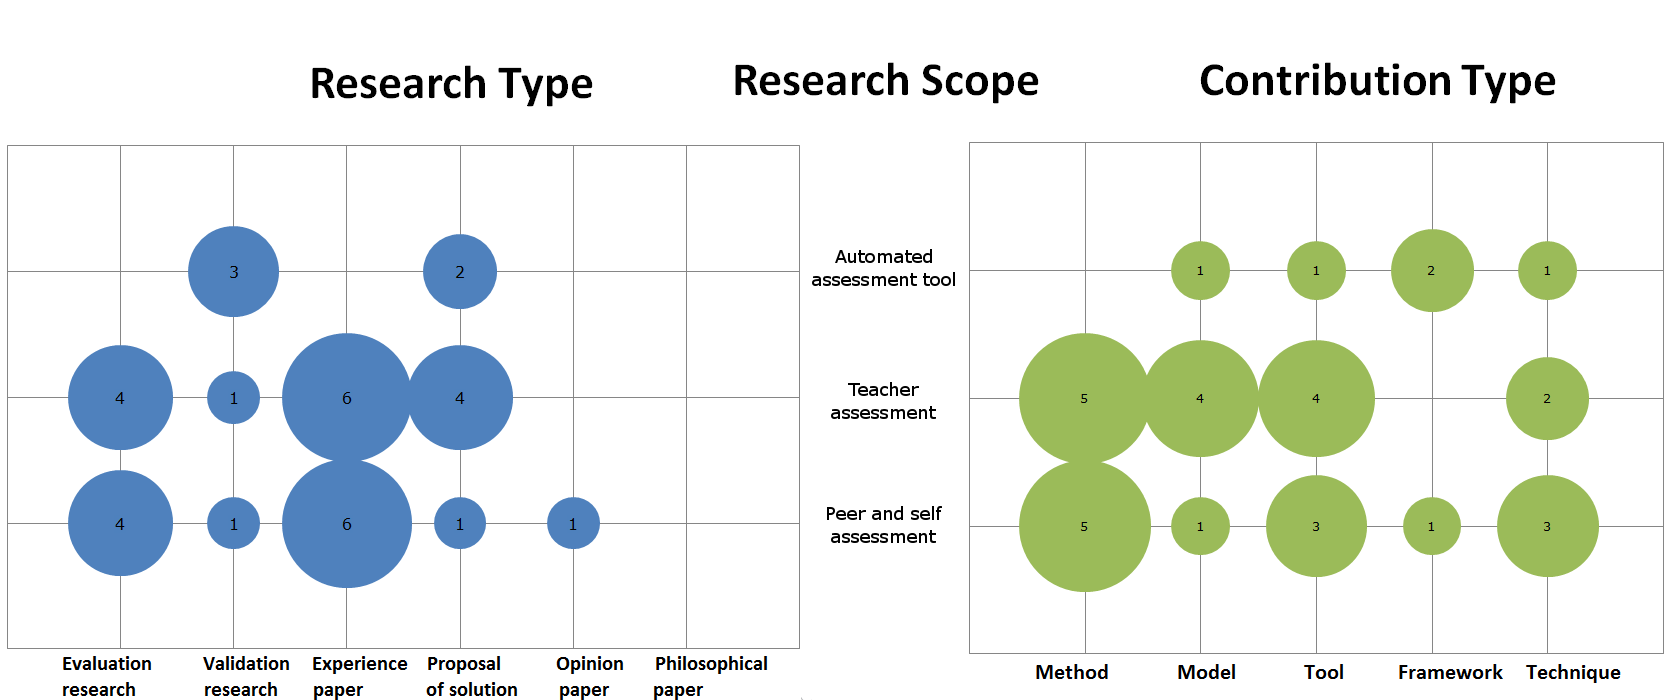
\includegraphics[scale=0.4]{BurbujasMargin.png}
  \end{center}
  \caption{Ámbito de trabajos distribuidos según tipo de investigación y según tipo de contribución}
  \label{fig:Burble}
\end{figure}
\end{landscape}
\pagestyle{fancy}

% Original pre-revision Juanma: EsquemaClasificacion.tex

\subsection{Esquema de clasificación}

Todos los artículos seleccionados comparten dos características: primero, que evalúan competencias genéricas y, segundo, que la tecnología juega un papel en esta evaluación. Este papel puede ser para el desarrollo de las competencias, para la evaluación de las mismas o para ambos. Para esta tesis el aspecto que nos interesa es la evaluación, aunque hay trabajos en los que no se puede separar el cómo se han trabajado las competencias de cómo se han evaluado. El listado de trabajos se muestra en la tabla~\ref{tab:ListadoTrabajos}.

Desde el punto de vista de la evaluación hay dos tipos de trabajos:
\begin{itemize}
\item Evaluación asistida: en este grupo se engloban trabajos en los que la función de la herramienta informática para la evaluación de una o varias competencias genéricas de los estudiantes es la de dar soporte a la misma proporcionando el formato para introducir datos (notas, indicadores, respuestas a preguntas, etc.). Pero necesitan que alguien introduzca dichos datos. En base a ese ``alguien`` nos encontramos dos tipos de trabajo:
	\begin{itemize}
		\item Autoevaluación o evaluación entre iguales.
		\item Evaluación del docente.
	\end{itemize}
\item Evaluación semiautomática: se utiliza una herramienta informática que automatiza en parte la evaluación de los estudiantes. Puede ser que esta herramienta requiera una intervención inicial del docente para introducir datos o configurar la propia herramienta.
\end{itemize}

\subsubsection*{Autoevaluación o evaluación entre iguales.}

La autoevaluación es un proceso en el que los estudiantes evalúan su propio trabajo, mientras que  en el proceso de evaluación entre iguales un estudiante evalúa el trabajo de otro u otros estudiantes. Esta práctica se emplea por un lado para mejorar tanto el conocimiento en la materia del alumnado como sus habilidades metacognitivas, y por otro, para aliviar la carga de trabajo del profesorado. A menudo este tipo de evaluación se acompaña de algún tipo de rúbrica~\cite{malehorn1994ten}.

En algunos trabajos el proceso de evaluación de competencias genéricas se lleva a cabo después de haber trabajado los estudiantes en actividades de un entorno virtual de aprendizaje mediante cuestionarios que completan los propios estudiantes o el docente. Los docentes confirman que el uso de herramientas web mejora la participación en la comunidad favoreciendo la colaboración y la construcción de conocimiento compartido~\cite{starcic2008sustaining}. Las herramientas que suelen utilizarse son wikis, foros, actividades y e-portfolio. Esta última aparece en varios trabajos, un e-portfolio (del inglés \emph{electronic portfolio}), consiste en un conjunto de documentos, generalmente textos, archivos e imágenes, gestionados en un entorno web por un usuario. Los estudiantes trabajan con esta herramienta durante el curso y al final autoevalúan el desempeño de alguna competencia genérica~\cite{arno2011promoting}. \nomenclature{e-portfolio}{Portfolio digital (electronic portfolio)}

Hay trabajos que implementan una metodología de \emph{aprendizaje basado en problemas} (PBL, del inglés \emph{Problem-Based Learning}) para desarrollar competencias específicas y genéricas en sus estudiantes y que después se evalúan mediante autoevaluación y evaluación entre iguales~\cite{martinez2014teamwork}. En \cite{lasa2013problem} los docentes llevaron a cabo la evaluación del 90\percentage{ }de las competencias utilizando la herramienta de rúbricas \emph{RubiStar}, mientras que los estudiantes mediante autoevaluación y evaluación entre iguales se encargaron del otro 10\percentage. \nomenclature{PBL}{Aprendizaje basado en problemas (Problem-Based Learning)}

En otro trabajos los estudiantes realizan una experiencia de \emph{aprendizaje basado en equipos} (TBL, del inglés \emph{Team-Based Learning}) utilizando algún tipo de herramienta colaborativa. En~\cite{ficapal2015learning} se presenta un modelo que persigue el aprendizaje basado en equipos para la adquisición y evaluación de competencias genéricas en un contexto de e-learning. Los estudiantes trabajaban en grupo y evaluaban su desempeño en el \emph{trabajo en equipo} mediante una rúbrica. La calificación se completó con un cuestionario. \nomenclature{TBL}{Aprendizaje basado en equipos (Team-Based Learning)}

Se encontraron varias experiencias que utilizan herramientas ligadas al ámbito empresarial (contabilidad, gestión de equipos, gestión de proyectos, etc.) que vienen acompañadas de rúbricas de autoevaluación.  En~\cite{chang2009international} se utiliza la herramienta Cycloid para el desarrollo de competencias en la gestión de proyectos y posteriormente se llevan a cabo autoevaluaciones de los propios estudiantes para valorar la adquisición de dichas competencias. También se autoevalúan competencias \emph{empresariales} en  \cite{achcaoucaou2014competence} mediante el uso de Tricuspoid.

Otra experiencia se lleva a cabo a partir de herramientas de videoconferencia como Skype o Hangouts. Los estudiantes realizan videoconferencias y después son autoevaluados o evaluados por sus compañeros en las competencias que deberían desempeñar en la actividad~\cite{masip2013self}.

A continuación se van a enumerar las competencias que se han evaluado, los métodos que se han seguido y las técnicas y herramientas que se han utilizado para llevar a cabo estas evaluaciones.

\paragraph*{- Competencias evaluadas}
Como se puede ver en la tabla~\ref{tab:CompetenciasAuto}, el \emph{trabajo en equipo} (6 trabajos) y la \emph{comunicación} (5 trabajos) son las competencias más evaluadas mediante evaluación entre iguales y autoevaluación. En el típico caso que encontramos en este grupo los estudiantes trabajan en grupo y evalúan su desempeño y el de sus compañeros en el \emph{trabajo en equipo} mediante una rúbrica~\cite{ficapal2015learning}.
El uso de tecnologías de la información (\emph{TIC}) y el \emph{idioma} son las otras competencias que destacan dentro de este grupo con 3 trabajos cada una. 

\begin{table}
  \begin{center}
  \begin{tabular}{| m{6cm} | c | m{5cm} |}
    \hline
    COMPETENCIA & CANT. & TRABAJOS\\
    \hline
    \hline
    Análisis & 2 & \cite{carreras2013promotion,lasa2013problem} \\
    \hline
    Aprendizaje permanente & 1 & \cite{oliver2013graduate} \\
    \hline
    Comunicación & 5 &  \cite{masip2013self,ruizacarate2013soft,carreras2013promotion,martinez2014teamwork,oliver2013graduate} \\
    \hline
    Creatividad & 1 & \cite{piedra2010measuring} \\
    \hline
    Cultural & 1 & \cite{oliver2013graduate} \\
    \hline
    Emprendimiento & 2 & \cite{chang2009international,achcaoucaou2014competence} \\
    \hline
    Gestión de proyectos & 1 & \cite{martinez2014teamwork} \\
    \hline
    Habilidades interpersonales & 1 & \cite{martinez2014teamwork} \\
    \hline
    Investigación & 1 & \cite{oliver2013graduate} \\
    \hline 
    Lengua extranjera & 3 & \cite{renau2010teaching,masip2013self,sevilla2012assessment} \\
    \hline
    Liderazgo & 1 & \cite{martinez2014teamwork} \\
    \hline
    Pensamiento crítico & 1 & \cite{arno2011promoting} \\
    \hline
    Planificación y gestión del tiempo & 1 & \cite{martinez2014teamwork} \\
    \hline
    Resolución de problemas & 1 & \cite{oliver2013graduate} \\
    \hline
    Responsabilidad & 2 & \cite{ruizacarate2013soft,carreras2013promotion} \\
    \hline
    TIC & 3 & \cite{lasa2013problem,masip2013self,oliver2013graduate} \\
    \hline
%    Toma de decisiones & 0 &   \\
%    \hline
    Trabajo autónomo & 1 &  \cite{lasa2013problem} \\
    \hline
    Trabajo en equipo & 6 &  \cite{lasa2013problem,ficapal2015learning,ruizacarate2013soft,piedra2010measuring,carreras2013promotion,martinez2014teamwork,oliver2013graduate} \\
    \hline
  \end{tabular}
\end{center}
\caption{Competencias genéricas evaluadas mediante autoevaluación y evaluación entre iguales}
\label{tab:CompetenciasAuto}
\end{table}

\paragraph*{- Métodos, técnicas e instrumentos de evaluación}
En la tabla~\ref{tab:MetodosAuto} se indican los métodos, técnicas e instrumentos de evaluación seguidas por cada uno de los trabajos que sigue este enfoque de autoevaluación y evaluación entre iguales. El método de evaluación más empleado es el sumativo (8 trabajos), mientras que las técnicas de observación sistemática y las pruebas escritas son los métodos más utilizados con 5 y 6 trabajos respectivamente, utilizando como herramientas cuestionarios y rúbricas. Podemos decir que el patrón clásico de este tipo de trabajos consiste en que los estudiantes se autoevalúan o evalúan a sus compañeros mediante rúbricas y cuestionarios una vez terminado el trabajo que debían realizar en el entorno virtual de aprendizaje. 

\begin{table}
  \begin{center}
  \begin{tabular}{| L{3cm} | L{3cm} | L{3.5cm} | L{2cm} |} % {| m{2cm} | m{4.5cm} | m{3cm} | m{2.5cm} |}   
    \hline
    MÉTODOS DE  & TÉCNICAS DE  & INSTRUMENTOS  & \multirow{2}{*}{TRABAJOS} \\
    EVALUACIÓN & EVALUACIÓN & DE EVALUACIÓN &  \\
    \hline
    \hline
    \multirow{4}{*}{Auténtica} & Actividades   & \multirow{2}{*}{-} & \multirow{2}{*}{\cite{renau2010teaching}} \\
     & sin determinar  &  &  \\
    \cline{2-4}
     & \multirow{2}{3cm}{Observación sistemática} & \multirow{2}{*}{Rúbrica} & \multirow{2}{*}{\cite{oliver2013graduate}} \\
     &  &  &  \\
    \hline
    \multirow{2}{*}{Formativa} & Pruebas escritas & Cuestionario & \cite{achcaoucaou2014competence}  \\
    \cline{2-4}
     & \multirow{2}{3cm}{Observación sistemática} & \multirow{3}{*}{Rúbrica} & \cite{arno2011promoting,piedra2010measuring} \\
    \cline{1-1} \cline{4-4}
    \multirow{3}{*}{Sumativa} &  &  & \cite{carreras2013promotion,lasa2013problem}  \\
    \cline{2-2} \cline{4-4}
     & Pruebas orales &  & \cite{masip2013self} \\
    \cline{2-4}
     & Pruebas escritas & Cuestionario & \cite{chang2009international,ficapal2015learning,martinez2014teamwork,ruizacarate2013soft,sevilla2012assessment} \\
    \hline
  \end{tabular}
\end{center}
\caption{Instrumentos de evaluación y métodos correspondientes a los trabajos de la autoevaluación y evaluación entre iguales}
\label{tab:MetodosAuto}
\end{table}

\paragraph*{- Análisis}
Aunque la autoevaluación y evaluación entre iguales son enfoques que pueden reducir el trabajo del docente, no siempre es así. En algunos trabajos anteriores, este enfoque a menudo sólo se utiliza de manera complementaria a algún otro tipo de evaluación~\cite{lasa2013problem,sevilla2012assessment}. Además, se puede dar el caso que la autoevaluación no se ajuste del todo a la realidad del desempeño del estudiante. Por ejemplo, en~\cite{carreras2013promotion} hay notables diferencias entre las calificaciones que se auto-asignan los estudiantes en algunas competencias y las calificaciones que le asignaron los docentes en esas mismas competencias. En ese trabajo se promovió la adquisición de competencias genéricas desde un punto de vista interdisciplinar y se diseñaron herramientas específicas para evaluar dichas habilidades. A la hora de evaluar, se realizaron tanto autoevaluaciones como evaluaciones del docente. En dicha experiencia se evaluaron cuatro competencias genéricas: \emph{capacidad de análisis},  \emph{habilidades de escritura}, \emph{responsabilidad} y \emph{capacidad de trabajo en equipo}. Cabe destacar discrepancias significativas entre las calificaciones que se auto-asignan los estudiantes en las dos primeras competencias. En la \emph{capacidad de análisis} la discrepancia es de un 55,65\percentage, mientras que en las \emph{habilidades de escritura} de un 13,75\percentage.


\subsubsection*{Evaluación del docente}

En esta sección se incluyen trabajos en los que la evaluación la realiza directamente el docente apoyándose en la tecnología. En su mayoría son trabajos en los que el docente ha de corregir cuestionarios con preguntas abiertas, en los que utiliza rúbricas para evaluar el trabajo de sus estudiantes en las herramientas del entorno virtual de aprendizaje o en los que evalúa competencias genéricas a partir de las calificaciones de los estudiantes en las actividades que han realizado durante el curso. 

En este tipo de trabajos se repiten experiencias ya vistas en la autoevaluación y evaluación entre iguales para la evaluación de competencias genéricas. Trabajos en los que la evaluación se realiza después de haber trabajado los estudiantes con herramientas del entorno virtual de aprendizaje~\cite{starcic2008sustaining}, metodologías PBL~\cite{lacuesta2009active} o experiencias basadas en videoconferencias~\cite{ward2011developing}.

En~\cite{yang2014fine} se implementa un itinerario de aprendizaje incluyendo la evaluación de competencias genéricas. Un itinerario de aprendizaje es un mapa conceptual que nos guía en el proceso de aprendizaje. En este tipo de trabajos se implementan los itinerarios de aprendizaje definiendo matemáticamente tanto las fórmulas necesarias para evaluar cada bloque del curso a partir de sus actividades como su combinación para evaluar los objetivos del curso y las competencias genéricas.

\paragraph*{- Competencias evaluadas}
Las competencia genérica más evaluada mediante la evaluación del docente es la \emph{comunicación} oral y escrita (6 trabajos). En estos trabajos los docentes evalúan a los estudiantes mediante la corrección de documentos escritos y presentaciones orales. También le siguen de cerca los trabajos que evalúan las competencias de \emph{trabajo en equipo} y de \emph{resolución de problemas} (5 trabajos cada una). En la tabla~\ref{tab:CompetenciasProfesor} puede ver la relación de competencias evaluadas y los trabajos.

\begin{table}
  \begin{center}
  \begin{tabular}{| m{6cm} | c | m{5cm} |}
    \hline
    COMPETENCIA & CANT. & TRABAJOS\\
    \hline
    \hline
    Análisis & 1 & \cite{aziz2007appraisal} \\
    \hline
    Aprendizaje permanente & 1 & \cite{rashid2008engineering} \\
    \hline
    Comunicación & 6 &  \cite{lacuesta2009active,martin2013acquired,rodriguez2010portfolio,benlloch2007adapting,yang2014fine,rashid2008engineering} \\
    \hline
%    Creatividad & 0 &  \\
%    \hline
%    Cultural & 0 &  \\
%    \hline
    Emprendimiento & 2 & \cite{ward2011developing,rashid2008engineering} \\
    \hline
%    Gestión de proyectos & 0 & \\
%    \hline
%    Habilidades interpersonales & 0 &  \\
%    \hline
%    Investigación & 0 &  \\
%    \hline
%    Liderazgo & 0 &  \\
%    \hline
    Pensamiento crítico & 2 & \cite{lacuesta2009active,aziz2007appraisal} \\
    \hline
    Planificación y gestión del tiempo & 1 & \cite{lacuesta2009active} \\
    \hline
    Resolución de problemas & 5 & \cite{martin2013acquired,rodriguez2010portfolio,benlloch2007adapting,vizcarro2013assessment,aziz2007appraisal} \\
    \hline
%    Responsabilidad & 0 &  \\
%    \hline 
%    Segundo idioma & 0 &  \\
%    \hline
%    TIC & 0 & \\
%    \hline
%    Toma de decisiones & 0 &   \\
%    \hline
    Trabajo autónomo & 1 &  \cite{lasa2013problem} \\
    \hline
    Trabajo en equipo & 5 &  \cite{lacuesta2009active,martin2013acquired,rodriguez2010portfolio,benlloch2007adapting,rashid2008engineering} \\
    \hline
  \end{tabular}
\end{center}
\caption{Competencias evaluadas directamente por el docente}
\label{tab:CompetenciasProfesor}
\end{table}
 
\paragraph*{- Métodos, Técnicas e instrumentos de evaluación}

Dentro de la evaluación del docente el método de evaluación más seguido vuelve a ser el sumativo (5 trabajos), seguido de cerca por el formativo (4 trabajos). La técnica más utilizada es la observación sistemática (6 trabajos) y la herramienta más utilizada, la rúbrica (4 trabajos). Puede verse el listado completo de métodos, herramientas y técnicas en la tabla~\ref{tab:MetodosProfesor}.

\begin{table}
  \begin{center}
  \begin{tabular}{| L{3cm} | L{3cm} | L{3.5cm} | L{2cm} |}
    \hline
    MÉTODOS DE  & TÉCNICAS DE  & INSTRUMENTOS  & \multirow{2}{*}{TRABAJOS} \\
    EVALUACIÓN & EVALUACIÓN & DE EVALUACIÓN &  \\
    \hline
    \hline
     Auténtica & \multirow{3}{3.5cm}{Actividades sin determinar} & \multirow{3}{*}{-}  & \cite{starcic2008sustaining} \\
    \cline{1-1} \cline{4-4}
     Con referencia &  &   & \multirow{2}{*}{\cite{serrano2013hiperion}} \\
     al criterio &  &   &  \\
    \hline
     \multirow{4}{*}{Formativa} & Pruebas orales & Entrevista & \cite{ward2011developing} \\
    \cline{2-4}
     & \multirow{4}{3.5cm}{Observación sistemática } & \multirow{2}{3.5cm}{Herramienta de seguimiento} & \multirow{2}{*}{\cite{benlloch2007adapting,lacuesta2009active}} \\
     &  &  & \\
    \cline{3-4}
      &  & \multirow{2}{*}{Rúbrica} & \cite{rodriguez2010portfolio} \\
    \cline{1-1} \cline{4-4}
     \multirow{4}{*}{Sumativa} &    &  & \cite{aziz2007appraisal,martin2013acquired,rashid2008engineering} \\
    \cline{2-4}
      & Actividades  & \multirow{2}{*}{-}  & \multirow{2}{*}{\cite{yang2014fine}} \\
      &  sin determinar &   &  \\
    \cline{2-4}
      & Pruebas escritas & Cuestionario & \cite{vizcarro2013assessment} \\
    \hline
    \end{tabular}
\end{center}
\caption{Instrumentos de evaluación y métodos correspondientes a los trabajos en los que la evaluación es realizada por los docentes}
\label{tab:MetodosProfesor}
\end{table} 

\paragraph*{- Análisis}
La escalabilidad es el problema más mencionado por los autores en los trabajos recopilados. En~\cite{serrano2013hiperion} se diseña \emph{Hiperion}, un sistema de recomendación que ayuda a diseñar actividades adaptadas a cada estudiante para mejorar sus competencias. En su estudio de caso los docentes evaluaban las competencias de los estudiantes manualmente y después aplicaban Hiperion. La principal desventaja de la herramienta es el tiempo que el docente ha de dedicar para asignar los diferentes logros y el peso de cada nota para cada competencia en las actividades. En línea con los problemas de escalabilidad anteriores nos encontramos con el trabajo mostrado en~\cite{lacuesta2009active}. En él se utiliza una metodología PBL, en la que se realiza una evaluación individualizada de cada estudiante y de cada grupo de estudiantes. El autor considera también que el esfuerzo necesario y carga de trabajo para cada docente es un poco mayor al habitual. Lo mismo ocurre en~\cite{benlloch2007adapting}, trabajo en el que los docentes concluyeron que el esfuerzo que realizaron fue excesivo a pesar de los buenos resultados obtenidos y descartaron el uso del portfolio para próximas experiencias ya que les supone una gran carga de trabajo sobre todo en el tramo final del curso.

\subsubsection*{Evaluación semiautomática}

Las herramientas de evaluación semiautomática son herramientas informáticas que ayudan al docente en el proceso de la evaluación automatizando dicho proceso y proporcionando una calificación o indicador para cada estudiante susceptible de ser aplicado a la evaluación de su desempeño en una o varias competencias genéricas. Estas herramientas requieren una intervención inicial del docente para introducir datos o configurar la herramienta. %Puede haber diferentes niveles de automatización dependiendo de cuánto tenga que intervenir el docente en el proceso. Un caso típico en el que los profesores han tratado de automatizar el proceso de evaluación se da en las asignaturas de programación en las titulaciones de informática. Un ejemplo de esto puede verse en~\cite{jackson2000semi}, trabajo del año 2000 en el que se muestra un software que prueba automáticamente todos los programas de los estudiantes, evitando que el profesor tenga que afrontar la tediosa tarea de ejecutar de uno en uno dichos programas. El sistema genera una serie de métricas y muestra al profesor finalmente el código fuente, para que éste pueda considerar y calificar otros aspectos relativos a la calidad que eran más difíciles de automatizar. Por otro lado en~\cite{vujovsevic2013software} tenemos un trabajo del año 2013 que muestra un software totalmente automático que evalúa los programas creados por los estudiantes desde tres perspectivas: funcionamiento, verificación y similitud con grafo de control de flujo.

En~\cite{andre2011formal} se propuso un modelo formal para asignar trabajadores a proyectos software. Para definir el modelo se siguió un método Delphi, donde un grupo de expertos definieron criterios para la evaluación de habilidades de trabajo en equipo y definieron un test psicológico.

Hay trabajos en los que se emplea una metodologia de aprendizaje basado en juegos (GBL, del inglés \emph{Game-Based Learning})~\cite{bedek2011behavioral,guenaga2013serious}. En ellos se utilizan juegos digitales con el fin de apoyar y mejorar la enseñanza, el aprendizaje y la evaluación. Se puede establecer como una actividad práctica donde los jugadores, a medida que van avanzado en las dinámicas del juego, deben evidenciar unas habilidades, conocimientos y competencias que muestran el alcance de los objetivos de aprendizaje~\cite{charlier2012not}. \nomenclature{GBL}{Aprendizaje basado en juegos (Game-Based Learning)}

Y finalmente se han encontrado trabajos que se basan en técnicas de \emph{learning analytics} para obtener indicadores con los que evaluar la competencia de trabajo en equipo a partir de la actividad de los estudiantes en diferentes entornos virtuales de aprendizaje~\cite{fidalgo:2015,rayon2014web}.

% El \emph{learning analytics} es definido por la \emph{Society for Learning Analytics} como la medición, recopilación, análisis y presentación de datos sobre los estudiantes, sus contextos y las interacciones que allí se generan, con el fin de comprender el proceso de aprendizaje que se está desarrollando y optimizar los entornos en los que se produce~\cite{siemens2012learning}.

\paragraph*{- Competencias evaluadas}
 En la tabla~\ref{tab:CompetenciasAutomaticas} se muestran las competencias evaluadas y los trabajos en que se evalúan. Aunque no son muchos trabajos los que encontramos en este grupo, cabe destacar que vuelve a ser la competencia de la \emph{comunicación} la más evaluada.

\begin{table}
  \begin{center}
  \begin{tabular}{| m{6cm} | c | m{5cm} |}
    \hline
    COMPETENCIA & CANT. & TRABAJOS\\
    \hline
    \hline
    Análisis & 1 & \cite{andre2011formal} \\
    \hline
    Aprendizaje permanente & 1 & \cite{andre2011formal}   \\
    \hline
    Comunicación & 3 & \cite{andre2011formal,rayon2014web,bedek2011behavioral}  \\
    \hline
    Creatividad & 1 & \cite{andre2011formal}   \\
    \hline
%    Cultural & 0 &  \\
%    \hline
    Emprendimiento & 1 & \cite{guenaga2013serious} \\
    \hline
    Gestión de proyectos & 1 & \cite{andre2011formal} \\
    \hline
    Habilidades interpersonales & 2 & \cite{andre2011formal,rayon2014web}  \\
    \hline
    Investigación & 1 & \cite{andre2011formal}  \\
    \hline
    Liderazgo & 1 & \cite{andre2011formal}  \\
    \hline
    Pensamiento crítico & 1 & \cite{andre2011formal} \\
    \hline
    Planificación y gestión del tiempo & 1 & \cite{andre2011formal} \\
    \hline
    Resolución de problemas & 1 & \cite{guenaga2013serious} \\
    \hline
    Responsabilidad & 1 & \cite{andre2011formal}  \\
    \hline 
%    Segundo idioma & 0 &  \\
%    \hline
%    TIC & 0 & \\
%    \hline
    Toma de decisiones & 1 & \cite{andre2011formal}   \\
    \hline
    Trabajo autónomo & 1 & \cite{andre2011formal} \\
    \hline
    Trabajo en equipo & 2 & \cite{andre2011formal,fidalgo:2015}  \\
    \hline
  \end{tabular}
\end{center}
\caption{Competencias evaluadas de forma semiautomática}
\label{tab:CompetenciasAutomaticas}
\end{table} 

\paragraph*{- Métodos, Técnicas e instrumentos de evaluación}
El método de evaluación formativo es el más empleado (3 trabajos). Al haber pocos trabajos no hay ninguna tendencia que destacar con respecto a las técnicas y las herramientas. Se puede ver cada método junto con las técnicas y herramientas empleadas en la tabla~\ref{tab:MetodosAutomaticos}.

\begin{table}
  \begin{center}
  \setlength\tabcolsep{2.5pt}
  \begin{tabular}{| m{2.7cm} | m{4cm} | m{4cm} | m{2cm} |}
    \hline 
    MÉTODOS DE  & TÉCNICAS DE  & INSTRUMENTOS  & \multirow{2}{*}{TRABAJOS} \\
    EVALUACIÓN & EVALUACIÓN & DE EVALUACIÓN &  \\
    \hline
    \hline
    Auténtico  & \multirow{2}{4cm}{Indicadores basados en logros} & \multirow{2}{*}{Juegos serios} & \cite{bedek2011behavioral} \\
    \cline{1-1} \cline{4-4}
    \multirow{4}{*}{Formativo} &  &  & \cite{guenaga2013serious} \\
    \cline{2-4}
     & \multirow{3}{4cm}{Indicadores de trabajo en entornos virtuales de aprendizaje} & \multirow{3}{4cm}{Herramienta para el análisis de los registros de aprendizaje} & \multirow{3}{*}{\cite{fidalgo:2015,rayon2014web}} \\
     &  &  &  \\
     &  &  &  \\
    \hline
    Sumativo & Pruebas escritas & Test automático & \cite{andre2011formal} \\
    \hline
  \end{tabular}
\end{center}
\caption{Instrumentos de evaluación y métodos correspondientes a los trabajos de evaluación semiautomática}
\label{tab:MetodosAutomaticos}
\end{table} 


\paragraph*{- Análisis}
La creación de los  tests de personalidad no está al alcance de todos los docentes. Como hemos visto antes en el trabajo presentado en~\cite{andre2011formal}, fue necesario llevar a cabo un modelo Delphi para la definición de los tests.

En \cite{guenaga2013serious} se utilizan los juegos serios para el desarrollo de las competencias de \emph{emprendimiento} y \emph{solución de problemas}. Se definieron una serie de indicadores como medida del desempeño en las competencias que permiten al estudiante conocer su nivel de adquisición de las mismas. En \cite{bedek2011behavioral} también se utilizan los juegos serios para el desarrollo y evaluación de competencias genéricas. Se basa en un modelo donde para cada competencia se identifican subcompetencias más específicas, lo que facilita el proceso de definición de indicadores. Los juegos serios suelen utilizarse con un propósito específico, generalmente relacionado con competencias específicas. Hay muchos trabajos sobre juegos serios en la literatura pero sólo dos que evalúen competencias genéricas. 

%También lo que para un profesor es un indicador del desempeño de competencias genéricas puede que no lo sea para otro, por lo que desarrollar un juego que sirva para todos los profesores es complicado %BUSCAR REFERENCIA

%Volvemos a encontrarnos con problemas de escalabilidad. El profesorado que participó en la experiencia de \cite{} reconoció que tuvieron que dedicar un elevado número de horas, tanto para las clases como para la evaluación de muchos proyectos. Más aún si los cuestionarios constan de preguntas abiertas y cerradas. Las preguntas abiertas obligan al evaluado a formular la respuesta a la pregunta y al evaluador a leerla para corregirla, lo que conlleva una mayor carga de trabajo. En \cite{} se presenta un cuestionario para evaluar el \emph{pensamiento crítico}, la \emph{curiosidad} y la \emph{creatividad}. El cuestionario consta sobre todo de preguntas abiertas, lo que implica tener que dedicar más tiempo y recursos para realizar las evaluaciones. En~\cite{vizcarro2013assessment}, profesores de los grados de Computación y Matemáticas y de Ingeniería Informática elaboraron una prueba escrita para la evaluación de la competencia genérica de \emph{resolución de problemas}. Este constaba de preguntas abiertas y cerradas, siendo minuciosamente seleccionadas por el profesorado que formaba parte en la experiencia, así como las respuestas que se esperarían de los estudiantes. El proyecto fue muy satisfactorio, aunque en las conclusiones vemos que los autores indican que encontrar un equilibrio entre el esfuerzo necesario para desarrollar este tipo de dispositivos de evaluación y la posibilidad de no hacerlo, o hacerlo pero no tan exhaustivamente, es algo que la comunidad académica debe abordar seriamente.


%En el trabajo presentado \cite{guenaga2013serious} se utilizan los juegos serios para el desarrollo y evaluación de las competencias de \emph{emprendimiento} y \emph{resolución de problemas}. En~\cite{rayon2014web} se evalúan competencias como la \emph{comunicación interpersonal} o las \emph{habilidades de escritura}. Y en \cite{fidalgo:2015} abordan la evaluación de la competencia de \emph{trabajo en equipo} (tabla~\ref{tab:CompetenciasAutomaticas}).



%En \cite{fidalgo:2015} también abordan la evaluación de la competencia de \emph{trabajo en equipo}. Pero en este caso se hace desde un enfoque completamente diferente. En este trabajo se propone utilizar indicadores basados en la interacción entre los agentes que intervienen en el proceso de aprendizaje: Mediante los mensajes escritos en el foro se mide la interacción estudiante-estudiante activo, mientras que mediante las lecturas en el foro se mide las interacciones estudiante-estudiante pasivo. En este trabajo los autores demuestran cómo estos indicadores están relacionados con el rendimiento trabajando en equipo de los estudiantes. Además, cómo la obtención de estos indicadores mediante los mecanismos de un entorno virtual es un trabajo tedioso y lento, se desarrolló en este mismo trabajo el software \emph{LA system (Learning Analytics system)}.

%En~\cite{rayon2014web} se propone la evaluación de varias competencias genéricas mediante indicadores obtenidos del análisis del proceso de aprendizaje. Para ello utilizan una plataforma web llamada LACAMOLC (\emph{Learning Analytics for Competence Assessment of MObile Learning Contexts}), un panel que da soporte a los procesos de aprendizaje y evaluación proporcionando una perspectiva visual del análisis del aprendizaje mediante la recolección de datos sociales y de uso desde diferentes entornos de aprendizaje como Moodle, Google Apps para la educación y MediaWiki. Mediante LACAMOLC el profesor centraliza todos los indicadores para la evaluación de competencias obteniendo una información cuantitativa y visual. Mediante el número de accesos al foro de Moodle o mediante el número de contribuciones en el foro, se evalúan competencias como la \emph{comunicación interpersonal} o las \emph{habilidades de escritura}. También se utilizan indicadores obtenidos de documentos Google (\emph{Google Docs}).

El primer trabajo en el que se usan los registros de actividad de los entornos de aprendizaje utiliza LACAMOLC, una plataforma web que aporta información visual e informes con indicadores de competencias genéricas de los estudiantes a partir de los registros de actividad~\cite{rayon2014web}. LACAMOLC está implementado sobre Pentaho. Pentaho es una herramienta de análisis de negocio que recoge datos de las bases de datos de los diferentes orígenes, y que mapeará estos datos con los indicadores de las competencias genéricas. Las competencias que se evalúan y los indicadores que se utilizan son:

\begin{itemize}
\item \emph{Gestión del tiempo}. Indicador: cumplimiento de la planificación, formulado en base al número de acciones que se han hecho a tiempo con respecto a la planificación fijada en una hoja de cálculo de Google Docs.
\item \emph{Comunicación interpersonal}. Indicador: escuchar a los demás, formulado en base al número de veces que los estudiantes accedieron a las discusiones del foro del LMS Moodle.
\item \emph{Comunicación interpersonal}. Indicador: expresar sus ideas, formulado en base a las intervenciones en el foro de Moodle y comentarios en un documento Google Docs.
\item \emph{Habilidades de escritura}. Indicador: expresar sus ideas, formulado en base al número de veces que cada estudiante intervino en los foros de Moodle dividido por el número de veces que accedió.
\item \emph{Habilidades de escritura}. Indicador: expresar sus ideas con claridad y precisión, formulado en base al número total de palabras que cada estudiante escribió dividido por el número de veces que intervino.
\item \emph{Trabajo en equipo}. Indicador: participación activa, formulado en base al tiempo total que duran las discusiones divididos por el número de sesiones.
\item \emph{Pensamiento analítico}. Indicador: respaldo de ideas de otros, formulado en base al número total de mensajes que un estudiante ha leído dividido entre el número de veces que intervino.
\item \emph{Pensamiento analítico}. Indicador: identificación de errores o falta de coherencia en sus propias ideas, formulado en base al número de veces que un estudiante releyó sus comentarios.
\end{itemize}

En el segundo trabajo que utiliza los registros de aprendizaje se utiliza el método CTMTC (\emph{Comprehensive Training Model of the Teamwork Competence}), que integra herramientas que están presentes en diferentes entornos virtuales de aprendizaje y que facilita el registro de la interacción de los estudiantes~\cite{fidalgo:2015}. El registro de esta interacción en el foro era una tarea tediosa para ser realizada a mano, por lo que implementaron el \emph{LA system}, un servicio web en Moodle, que permite que la información sea accesible a través de internet con mensajes basados en XML. Esta información después es consumida por un cliente que visualiza los datos. Los indicadores utilizados para evaluar el trabajo en equipo son: \nomenclature{CTMTC}{Comprehensive Training Model of the Teamwork Competence}

\begin{itemize}
\item Mensajes escritos en foro: interacción estudiante-estudiante activo.
\item Mensajes leídos en el foro:  interacciones estudiante-estudiante pasivo.
\end{itemize}

Estos dos trabajos proporcionan indicadores de los entornos virtuales de aprendizaje aplicables a varias competencias genéricas. El inconveniente que presentan ambas aproximaciones es que los indicadores son fijos, es decir, el docente no tendría la opción de combinar o buscar otros indicadores en el entorno virtual aparte de los que proporcionan los métodos presentados. Por ejemplo, si en un LMS se utilizan los foros con unas reglas de uso diferentes quizás habría que modificar los indicadores o combinarlos de otra manera para que fueran útiles para el docente. Sería deseable la opción de que el docente pudiera diseñar sus propias evaluaciones a partir de los indicadores que proporciona el entorno virtual de aprendizaje.

\begin{landscape}
\pagestyle{empty}
\begin{center}
  \setlength\tabcolsep{3.5pt}
\begin{longtable}{| c | L{9cm} | L{3.7cm} | L{3.1cm} | L{3.5cm} |}
    \hline
    \multirow{2}{*}{REF} & \multirow{2}{*}{TÍTULO} &  TIPO DE  &  TIPO DE  &  ÁMBITO DE LA  \\
     &  &  INVESTIGACIÓN &   CONTRIBUCIÓN &   INVESTIGACIÓN \\
    \hline
    \hline 
    \cite{yang2014fine} & A Fine-Grained Outcome-Based Learning Path Model & proposal of solution & model & Teacher assessment \\
    \hline
    \cite{rayon2014web} & A web platform for the assessment of competences in Mobile Learning Contexts & validation research & framework & \leftcell{3.8cm}{Automated assessment tool} \\
    \hline
    \cite{martin2013acquired} & Acquired Skills With The Implementation Of New Evaluation Methods At University Rey Juan Carlos & experience paper & model & Teacher assessment \\
    \hline
    \cite{lacuesta2009active} & Active learning through problem based learning methodology in engineering education & experience paper & method & Teacher assessment \\
    \hline
    \cite{benlloch2007adapting} & Adapting teaching and assessment strategies to enhance competence-based learning in the framework of the european convergence process & proposal of solution & method & Teacher assessment \\
    \hline
    \cite{aziz2007appraisal} & Appraisal of Course Learning Outcomes using Rasch Measurement: A Case Study in Information Technology Education & proposal of solution & model & Teacher assessment \\
    \hline
    \cite{sevilla2012assessment} & Assessment of competences in designing online preparatory materials for the Cambridge First Certificate in English examination & evaluation research & technique & \leftcell{3.8cm}{Peer and self-assessment / Teacher assessment} \\
    \hline
    \cite{vizcarro2013assessment} & Assessment of problem solving in computing studies & experience paper & method & Teacher assessment \\
    \hline
    \cite{achcaoucaou2014competence} & Competence Assessment in Higher Education: A Dynamic Approach & proposal of solution & tool & \leftcell{3.8cm}{Peer and self-assessment} \\
    \hline
    \cite{strijbos2015criteria} & Criteria and standards of generic competences at bachelor degree level: A review study & evaluation research & method & Review study \\
    \hline
    \cite{ward2011developing} & Developing entrepreneurial accounting and finance competency using the ELLEIEC Virtual Centre for Enterprise & experience paper & tool & Teacher assessment \\
    \hline
    \cite{ficapal2015learning} & e-Learning and Team-based Learning. Practical Experience in Virtual Teams & experience paper & framework & \leftcell{3.8cm}{Peer and self-assessment} \\
    \hline
    \cite{rashid2008engineering} & Engineering Students Performance Evaluation of Generic Skills Measurement: ESPEGS Model & validation research & model & Teacher assessment \\
    \hline
    \cite{rodriguez2010portfolio} & e-Portfolio: A tool to assess university students' skills & evaluation research & tool & Teacher assessment \\
    \hline
    \cite{andre2011formal} & Formal model for assigning human resources to teams in software projects & validation research & model & \leftcell{3.8cm}{Automated assessment tool} \\
    \hline
    \cite{bedek2011behavioral} & From Behavioral Indicators to Contextualized Competence Assessment & proposal of solution & framework & \leftcell{3.8cm}{Automated assessment tool} \\
    \hline
    \cite{oliver2013graduate} & Graduate attributes as a focus for institution-wide curriculum renewal: innovations and challenges & opinion paper & model & \leftcell{3.8cm}{Peer and self-assessment} \\
    \hline
    \cite{serrano2013hiperion} & Hiperion: A fuzzy approach for recommending educational activities based on the acquisition of competences & proposal of solution & tool & Teacher assessment \\
    \hline
    \cite{chang2009international} & International creative tension study of university students in South Korea and Finland & evaluation research & tool & \leftcell{3.8cm}{Peer and self-assessment} \\
    \hline
    \cite{piedra2010measuring} & Measuring collaboration and creativity skills through rubrics: Experience from UTPL collaborative social networks course & evaluation research & method & \leftcell{3.8cm}{Peer and self-assessment / Teacher assessment} \\
    \hline
    \cite{lasa2013problem} & Problem Based Learning Implementation In The Degree Of Human Nutrition And Dietetics & experience paper & technique & \leftcell{3.8cm}{Peer and self-assessment / Teacher assessment} \\
    \hline
    \cite{arno2011promoting} & Promoting reflection on science, technology, and society among engineering students through an EAP online learning environment & evaluation research & tool & \leftcell{3.8cm}{Peer and self-assessment} \\
    \hline
    \cite{masip2013self} & Self-video recording for the integration and assessment of generic competencies & experience paper & technique & \leftcell{3.8cm}{Peer and self-assessment} \\
    \hline
    \cite{guenaga2013serious} & Serious Games for the Development of Employment Oriented Competences & validation research & tool & \leftcell{3.8cm}{Automated assessment tool} \\
    \hline
    \cite{ruizacarate2013soft} & Soft Skills: A Comparative Analysis Between Online and Classroom Teaching & experience paper & method & \leftcell{3.8cm}{Peer and self-assessment} \\
    \hline
    \cite{starcic2008sustaining} & Sustaining Teacher's Professional Development and Training through Web-Based Communities of Practice & evaluation research & tool & Teacher assessment \\
    \hline
    \cite{renau2010teaching} & Teaching And Learning Through Projects Using The ICT: Practice Of The English Writing Through Business Documents & experience paper & method & \leftcell{3.8cm}{Peer and self-assessment} \\
    \hline
    \cite{martinez2014teamwork} & Teamwork competence and academic motivation in computer science engineering studies & validation research & method & \leftcell{3.8cm}{Peer and self-assessment} \\
    \hline
    \cite{carreras2013promotion} & The promotion and assessment of generic skills from interdisciplinary teaching teams & experience paper & method & \leftcell{3.8cm}{Peer and self-assessment / Teacher assessment} \\
    \hline
    \cite{fidalgo:2015} & Using Learning Analytics to improve teamwork assessment & proposal of solution & technique & \leftcell{3.8cm}{Automated assessment tool} \\
    \hline
\caption{Distribución de publicaciones por tratamiento del problema}
\label{tab:ListadoTrabajos}
\end{longtable}
\end{center}
\end{landscape}

\pagestyle{fancy}
\section{Respuestas a las preguntas de investigación}

En base al estudio las respuestas a las preguntas de investigación son las siguientes:

\paragraph*{Q1. ¿Qué competencias se han evaluado de forma automática o asistida por ordenador  a partir de la actividad de los estudiantes en los entornos virtuales de aprendizaje?}

%  \, = mini espacios metidos para provocar que la frase ocupe una línea más porque quedeba feo en el pdf. Para comprobar lo que digo, quitarlos, compilar y ver.

En esta selección de trabajos se han encontrado evaluaciones para todas las competencias que fueron definidas en la tabla~\ref{tab:CompetenciasGenericas}. Aunque las más evaluadas son la \emph{comunicación} (14 trabajos), \emph{trabajo en equipo} (13 trabajos) y \emph{resolución de problemas} (7 trabajos). El resumen completo de número de trabajos por competencia puede verse en la tabla~\ref{tab:TrabajosCompetencia}.

Estos datos se pueden contrastar con los de la revisión de la literatura mostrada en \cite{strijbos2015criteria}, donde se analizan las competencias genéricas más frecuentemente evaluadas. En este caso repite primera posición la competencia de la \emph{comunicación}. La competencia de \emph{resolución de problemas} ocupa la cuarta posición, mientras que la de \emph{trabajo en equipo} pasa a sexto lugar. En esta revisión de la literatura se hallaron más artículos para todas las competencias, ya que no se descartaron por no ser procesos soportados tecnológicamente. El hecho de que haya más trabajos en proporción para la competencia de \emph{trabajo en equipo} en nuestra selección de trabajos se puede deber a que los entornos virtuales de aprendizaje modernos suelen favorecer los procesos de cooperación~\cite{i2007competencias}.

% , siendo la competencia de \emph{procesamiento de la información} es la que ocupa la segunda plaza

\begin{table}
  \begin{center}
  \begin{tabular}{| m{10cm} | c |}
    \hline
    COMPETENCIA & TRABAJOS\\
    \hline
    \hline
    Análisis & 4\\
    \hline
    Aprendizaje permanente & 3\\
    \hline
    Comunicación & 14\\
    \hline
    Creatividad & 3\\
    \hline
    Cultural & 1\\
    \hline
    Emprendimiento & 5\\
    \hline
    Gestión de proyectos & 2\\
    \hline
    Habilidades interpersonales & 3\\
    \hline
    Investigación & 2\\
    \hline 
    Lengua extranjera & 3\\
    \hline
    Liderazgo & 2\\
    \hline
    Pensamiento crítico & 4\\
    \hline
    Planificación y gestión del tiempo & 3\\
    \hline
    Resolución de problemas & 7\\
    \hline
    Responsabilidad & 3\\
    \hline
    TIC & 3\\
    \hline
    Toma de decisiones & 1\\
    \hline
    Trabajo autónomo & 2\\
    \hline
    Trabajo en equipo & 13\\
    \hline
  \end{tabular}
\end{center}
\caption{Número de trabajos que evalúan cada competencia genérica}
\label{tab:TrabajosCompetencia}
\end{table} 

\paragraph*{Q2. ¿Qué métodos se utilizan para evaluar competencias genéricas en entornos virtuales de aprendizaje?}

Se han encontrado dos grupos de trabajo, por un lado, aquellos en los que el entorno virtual de aprendizaje asiste al usuario en la evaluación, y por el otro, aquellos en los que el entorno virtual de aprendizaje realiza la evaluación automáticamente. Dentro del primer grupo, estos trabajos se dividen en dos subgrupos dependiendo de quién realice la evaluación: evaluación entre iguales o autoevaluación (cuando la evaluación la realizan los estudiantes) y evaluación del docente.

Estos grupos se han separado en la categorización final debido al elevado número de trabajos que hay para cada uno de ellos. Además, las competencias que se evalúan no son las mismas con un enfoque u otro. Mientras que ambos enfoques tienen un número elevado de trabajos que evalúan las competencias de \emph{comunicación} y \emph{trabajo en equipo}, la competencia de \emph{resolución de problema} tiene una presencia mucho más significativa en trabajos en los que evalúa el docente (5 trabajos) con respecto a trabajos que evalúan los estudiantes (1 trabajo).

La herramienta que más se utiliza tanto en la evaluación del docente como en la evaluación entre iguales o autoevaluación es la rúbrica electrónica. El problema que encontramos es estos trabajos que utilizan rúbricas es que si el docente se encarga de la evaluación, la carga de trabajo de éste aumenta~\cite{lacuesta2009active}. Sin embargo, si se delega en la autoevaluación o evaluación entre iguales pueden aparecer discrepancias entre las calificaciones que se auto-asignan los estudiantes y las que reciben por otros medios~\cite{carreras2013promotion}. 

Dentro de la evaluación semiautomática se seleccionaron 5 trabajos, entre los que se encuentran algunos basados en juegos serios~\cite{djaouti2011classifying,bedek2011behavioral} y otros basados en el análisis de los procesos de aprendizaje~\cite{rayon2014web,fidalgo:2015}.

Pueden verse las competencias genéricas evaluadas con cada método en las figuras~\ref{fig:competencias1} y~\ref{fig:competencias2}.

\begin{landscape}
\pagestyle{empty}
\begin{figure}[h]
  \begin{center}
    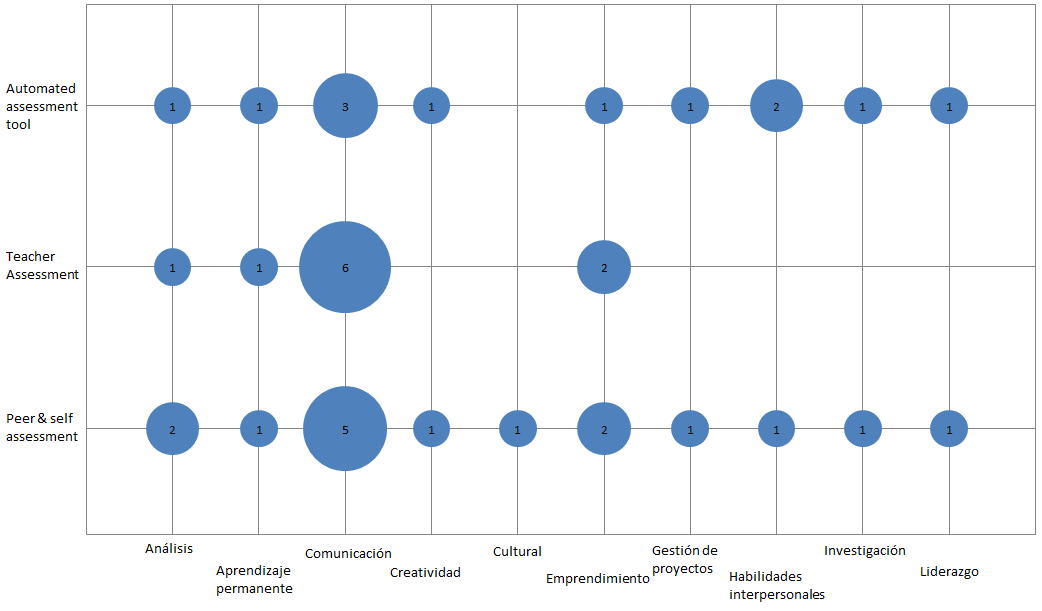
\includegraphics[scale=0.6]{BurbujaCompetenciasCut1.png}
  \end{center}
  \caption{Competencias genéricas evaluadas con cada método (1 de 2)}
  \label{fig:competencias1}
\end{figure}

\begin{figure}[h]
  \begin{center}
    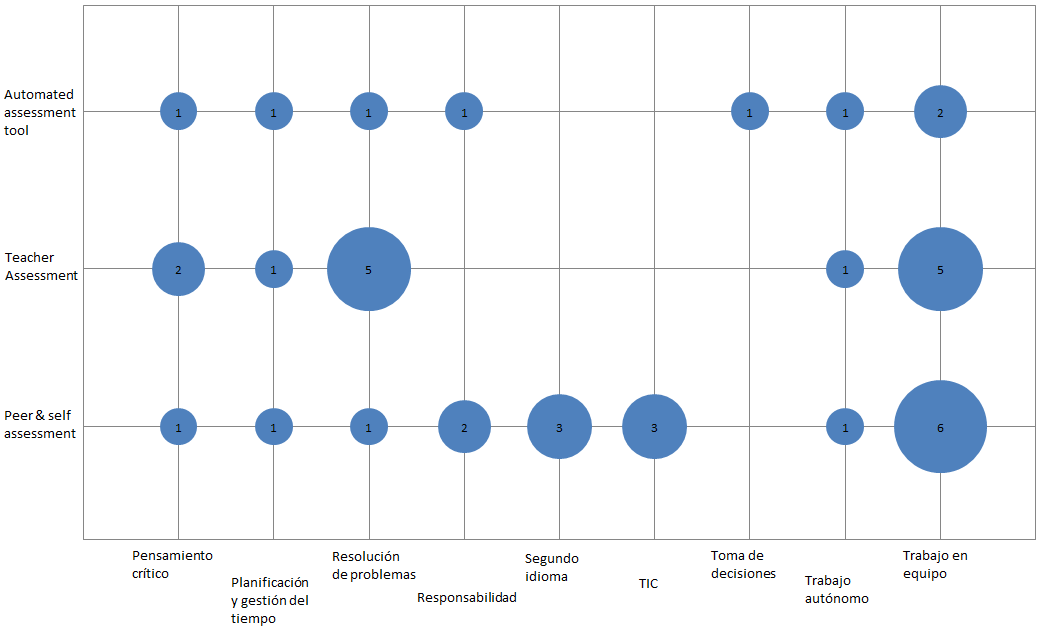
\includegraphics[scale=0.6]{BurbujaCompetenciasCut2.png}
  \end{center}
  \caption{Competencias genéricas evaluadas con cada método (2 de 2)}
  \label{fig:competencias2}
\end{figure}

\end{landscape}
\pagestyle{fancy}

\paragraph*{Q3. ¿Qué técnicas se utilizan para evaluar competencias genéricas a partir de los registros de actividad de un entorno virtual de aprendizaje?}

Dentro de los trabajos que realizan una evaluación semiautomática hay dos trabajos que utilizan un método de evaluación formativo a partir de técnicas para la extracción de indicadores de trabajo en el entorno virtual de aprendizaje utilizando herramientas para el análisis de los registros de aprendizaje~\cite{rayon2014web,fidalgo:2015}. 

En~\cite{rayon2014web} se utilizan procesos ETL (Extract, Transform and Load) mediante el uso de la herramienta de análisis Pentaho para obtener los registros de actividad de diversos KLT (Knowledge and Learning Technologies) como Moodle, Google Apps for Education, Mediawiki y Edmondo.

En~\cite{fidalgo:2015} se utilizan procesos de minería de datos (\emph{data mining}) mediante el desarrollo de un servicio web en Moodle que devuelve información almacenada en los registros en la plataforma de aprendizaje.

A continuación se muestra un resumen para estos trabajos indicando las técnicas empleadas, los métodos aplicados y las competencias evaluadas (tabla~\ref{tab:CompetenciasMetodosTecnicas}).

\begin{table}[h]
  \begin{center}
  \setlength\tabcolsep{2.5pt}
  \begin{tabular}{| l | c | c | c |}
    \hline
     \multirow{4}{*}{\textbf{Competencias}} & \textbf{Métodos} & \textbf{Técnicas} 		& \textbf{Herramientas} \\
    \cline{2-4}
     & \multirow{3}{*}{Formativo}  & \multirow{3}{4cm}{Indicadores de trabajo en entornos virtuales de aprendizaje} & \multirow{3}{3.9cm}{Herramienta para el análisis de los registros de aprendizaje} \\
     &   								&  															& \\
     &   								&  															&  \\
    \hline
    \hline
    \emph{Análisis} & \multicolumn{3}{c|}{ \multirow{6}{*}{\cite{rayon2014web} }}  \\
    \cline{1-1}
    \emph{Comunicación} & \multicolumn{3}{c|}{}  \\
    \cline{1-1}
    \multirow{2}{3cm}{\emph{\centering Habilidades interpersonales}} & \multicolumn{3}{c|}{} \\
     & \multicolumn{3}{c|}{} \\
    \cline{1-1}
    \emph{Planificación} & \multicolumn{3}{c|}{}  \\
    \cline{1-1}
    \multirow{2}{*}{\emph{Trabajo en equipo}} & \multicolumn{3}{c|}{} \\
    \cline{2-4}
     & \multicolumn{3}{c|}{\cite{fidalgo:2015}}  \\
    \hline
  \end{tabular}
\end{center}
\caption{Competetencias evaluadas, métodos aplicados y técnicas seguidas para evaluar competencias a partir de los registros de actividad de los entornos de aprendizaje}
\label{tab:CompetenciasMetodosTecnicas}
\end{table}

\section{Conclusiones}

Las competencias genéricas son hoy en día una pieza fundamental en las planificaciones de la enseñanza a todos los niveles académicos. Como consecuencia de esto, son numerosos los trabajos y los proyectos que se han puesto en marcha en los últimos años para fomentar el desarrollo de las mismas en los estudiantes. Tanto durante el desarrollo como a la finalización de estos trabajos y proyectos, es deseable una evaluación del nivel de adquisición de estas competencias en los estudiantes.

En la literatura hemos encontrado diferentes problemas a la hora de afrontar esta evaluación. Por un lado problemas de objetividad, ya que los criterios que para un docente son válidos para la evaluación de una competencia genérica pueden no ser válidos para otro. Y por otro lado, problemas de escalabilidad. Si ya en muchos casos la carga de trabajo del profesorado para poder alcanzar los objetivos del curso es elevada, aún más lo será si éstos tienen además que generar y evaluar nuevas actividades para medir el nivel de desempeño de sus estudiantes en competencias genéricas. Es más, este problema de escalabilidad se acrecienta en el contexto de los LMS, donde los cursos en ocasiones contienen un número muy elevado de estudiantes (por ejemplo los cursos de tipo MOOC).

Para conocer el estado del arte en la evaluación de competencias genéricas mediante el uso de la tecnología se ha realizado un estudio de la literatura en forma de SMS. Tras esta revisión fueron 30 los trabajos seleccionados y a partir de ellos se ha dado respuesta a las preguntas de investigación inicialmente planteadas.

En muchos de estos trabajos es el docente quien realiza la evaluación apoyándose en diferentes herramientas, pero estos trabajos suelen presentar problemas de escalabilidad. También tenemos trabajos en los que se trata de minimizar esta carga de trabajo del docente combinando o sustituyendo la evaluación del docente con evaluaciones entre iguales o autoevaluaciones. Esto evita en parte el problema de la carga de trabajo, pero nos encontramos con problemas de objetividad en algunas evaluaciones de los estudiantes. Como consecuencia, el profesorado tiene que revisar las evaluaciones de sus estudiantes, por lo que se puede volver a encontrar con problemas de carga de trabajo.

Otros trabajos consisten en la implementación de alguna herramienta online de cuestionarios de personalidad, normalmente diseñados para revelar aspectos del carácter o mecanismos psicológicos de un individuo. El inconveniente es que realizar un cuestionario de este tipo no está al alcance de cualquier docente, sino que debe tener formación en psicología, especialmente para diagnosticar o valorar los resultados. Y aunque se trate de automatizar el procedimiento, en ocasiones estos tests están formados con preguntas cerradas y abiertas, y en el caso de estas últimas, volvemos a encontrarnos con problemas de escalabilidad.

Por último hemos encontrado un conjunto de trabajos que automatizan el proceso de evaluación de competencias genéricas. Por un lado encontramos juegos serios, juegos que emulan un caso real profesional y en base al modo de actuar del estudiante obtendrán una puntuación que servirá como medida del desempeño en ciertas competencias. Estos juegos suelen estar muy enfocados a ciertas competencias no genéricas y su implementación es costosa. Además, el proceso de extracción de calificaciones no está automatizado ni integrado con las herramientas de evaluación del docente, por lo que es necesario un procedimiento manual para capturarlas.

Por otro lado nos encontramos con el tipo de trabajo que cubren en mayor medida los objetivos de nuestra investigación: trabajos que evalúan competencias genéricas a partir de indicadores obtenidos de los registros de los entornos de aprendizaje. En estos trabajos las herramientas proporcionan unos indicadores fijos sobre actividades concretas, pero no dan al docente la opción de decidir fórmulas ni crear sus propias evaluaciones, así que lo que proporciona la herramienta podría ser válido para un docente pero no serlo para otro. Si tuviéramos un método que nos permitiera diseñar evaluaciones se podrían probar diferentes fórmulas para obtener diferentes indicadores del desempeño de los estudiantes en el entorno virtual de aprendizaje hasta encontrar aquellos que se adapten a lo que cada docente considere válido para la evaluación de competencias.

\pagestyle{fancy}


% ----------------------------------------------------------------------

